%Version 3 October 2023
% See section 11 of the User Manual for version history
%
%%%%%%%%%%%%%%%%%%%%%%%%%%%%%%%%%%%%%%%%%%%%%%%%%%%%%%%%%%%%%%%%%%%%%%
%%                                                                 %%
%% Please do not use \input{...} to include other tex files.       %%
%% Submit your LaTeX manuscript as one .tex document.              %%
%%                                                                 %%
%% All additional figures and files should be attached             %%
%% separately and not embedded in the \TeX\ document itself.       %%
%%                                                                 %%
%%%%%%%%%%%%%%%%%%%%%%%%%%%%%%%%%%%%%%%%%%%%%%%%%%%%%%%%%%%%%%%%%%%%%

%%\documentclass[referee,sn-basic]{sn-jnl}% referee option is meant for double line spacing

%%=======================================================%%
%% to print line n      umbers in the margin use lineno option %%
%%=======================================================%%

%%\documentclass[lineno,sn-basic]{sn-jnl}% Basic Springer Nature Reference Style/Chemistry Reference Style

%%======================================================%%
%% to compile with pdflatex/xelatex use pdflatex option %%
%%======================================================%%

%%\documentclass[pdflatex,sn-basic]{sn-jnl}% Basic Springer Nature Reference Style/Chemistry Reference Style


%%Note: the following reference styles support Namedate and Numbered referencing. By default the style follows the most common style. To switch between the options you can add or remove �Numbered� in the optional parenthesis. 
%%The option is available for: sn-basic.bst, sn-vancouver.bst, sn-chicago.bst%  
 
%%\documentclass[sn-nature]{sn-jnl}% Style for submissions to Nature Portfolio journals
%%\documentclass[sn-basic]{sn-jnl}% Basic Springer Nature Reference Style/Chemistry Reference Style
\documentclass[pdflatex,sn-mathphys-num]{sn-jnl}% Math and Physical Sciences Numbered Reference Style 
%%\documentclass[sn-mathphys-ay]{sn-jnl}% Math and Physical Sciences Author Year Reference Style
%%\documentclass[sn-aps]{sn-jnl}% American Physical Society (APS) Reference Style
%%\documentclass[sn-vancouver,Numbered]{sn-jnl}% Vancouver Reference Style
%%\documentclass[sn-apa]{sn-jnl}% APA Reference Style 
%%\documentclass[sn-chicago]{sn-jnl}% Chicago-based Humanities Reference Style

%%%% Standard Packages
%%<additional latex packages if required can be included here>

\usepackage{graphicx}%
\usepackage{multirow}%
\usepackage{amsmath,amssymb,amsfonts}%
\usepackage{amsthm}%
\usepackage{mathrsfs}%
\usepackage[title]{appendix}%
\usepackage{xcolor}%
\usepackage{textcomp}%
\usepackage{manyfoot}%
\usepackage{booktabs}%
\usepackage{placeins}%

\usepackage{listings}%

\usepackage{amsmath,amsfonts,amsbsy,amssymb,mathtools,amsthm,tabulary,graphicx,times,caption,fancyhdr, mathrsfs, pgf, epsfig, epstopdf, lscape, subfig,booktabs, enumitem,lipsum,tkz-graph,scalerel,stackengine,setspace,kbordermatrix,algpseudocode, algorithm, accents, verbatim, dsfont}



% put your definitions there:

\newlength{\depthofsumsign}
\setlength{\depthofsumsign}{\depthof{$\sum$}}
\newlength{\totalheightofsumsign}
\newlength{\heightanddepthofargument}

\newcommand{\nsum}[1][1.4]{% only for \displaystyle
	\mathop{%
		\raisebox
		{-#1\depthofsumsign+1\depthofsumsign}
		{\scalebox
			{#1}
			{$\displaystyle\sum$}%
		}
	}
}




\GraphInit[vstyle = Shade]
\usetikzlibrary{decorations.pathreplacing}
\tikzset{
	LabelStyle/.style = { rectangle, rounded corners, draw,
		minimum width = 2em, fill = yellow!50,
		text = red, font = \Large\bfseries },
	VertexStyle/.append style = { inner sep=5pt,
		font = \Large\bfseries},
	EdgeStyle/.append style = {->, bend left} }




\tikzset{
	mynode/.style={
		draw,
		thick,
		anchor=south west,
		minimum width=2cm,
		minimum height=1.3cm,
		align=center, 
		inner sep=0.2cm,
		outer sep=0,
		rectangle split, 
		rectangle split parts=2,
		rectangle split draw splits=false},
	reverseclip/.style={
		insert path={(current page.north east) --
			(current page.south east) --
			(current page.south west) --
			(current page.north west) --
			(current page.north east)}
	}
}

\tikzstyle{io} = [trapezium, trapezium left angle=70, trapezium right angle=110, minimum width=3cm, minimum height=0.5cm, text centered, draw=black, fill=gray!10]
\tikzstyle{process} = [rectangle, minimum width=3cm, minimum height=1cm, text centered, draw=black, fill=gray!20]
\tikzstyle{process2} = [rectangle, minimum width=3cm, minimum height=1cm, text centered, draw=black, fill=gray!15]
\tikzstyle{process3} = [rectangle, minimum width=2cm, minimum height=1cm, text centered, draw=black, fill=gray!25]

\newcommand{\MaxNumberX}{3}
\newcommand{\MaxNumberY}{5}


\newcommand{\CommaBin}{\mathbin{\raisebox{0.5ex}{,}}}
\newcommand{\CommaPunct}{\mathpunct{\raisebox{0.5ex}{,}}}



\renewcommand\qedsymbol{$\blacksquare$}

\newcommand{\blue}[1]{\textcolor{blue}{#1}}




\DeclareFontFamily{U}{mathx}{\hyphenchar\font45}
\DeclareFontShape{U}{mathx}{m}{n}{
	<-6> mathx5 <6-7> mathx6 <7-8> matha7
	<8-9> mathx8 <9-10> mathx9
	<10-12> mathx10 <12-> mathx12
}{}
\DeclareSymbolFont{mathx}{U}{mathx}{m}{n}
\DeclareMathSymbol{\bigominus}{\mathop}{mathx}{"C1}








\DeclareMathAlphabet\mathbfcal{OMS}{cmsy}{b}{n}  
\DeclareMathOperator*{\argmax}{argmax}
\DeclareMathOperator*{\argmin}{argmin}

\stackMath
\newcommand\reallywidehat[1]{%
	\savestack{\tmpbox}{\stretchto{%
			\scaleto{%
				\scalerel*[\widthof{\ensuremath{#1}}]{\kern-.6pt\bigwedge\kern-.6pt}%
				{\rule[-\textheight/2]{1ex}{\textheight}}%WIDTH-LIMITED BIG WEDGE
			}{\textheight}% 
		}{0.5ex}}%
	\stackon[1pt]{#1}{\tmpbox}%
}

%%%%

%%%%%=============================================================================%%%%
%%%%  Remarks: This template is provided to aid authors with the preparation
%%%%  of original research articles intended for submission to journals published 
%%%%  by Springer Nature. The guidance has been prepared in partnership with 
%%%%  production teams to conform to Springer Nature technical requirements. 
%%%%  Editorial and presentation requirements differ among journal portfolios and 
%%%%  research disciplines. You may find sections in this template are irrelevant 
%%%%  to your work and are empowered to omit any such section if allowed by the 
%%%%  journal you intend to submit to. The submission guidelines and policies 
%%%%  of the journal take precedence. A detailed User Manual is available in the 
%%%%  template package for technical guidance.
%%%%%=============================================================================%%%%

%% as per the requirement new theorem styles can be included as shown below
\theoremstyle{thmstyleone}%
\newtheorem{theorem}{Theorem}%  meant for continuous numbers
%%\newtheorem{theorem}{Theorem}[section]% meant for sectionwise numbers
%% optional argument [theorem] produces theorem numbering sequence instead of independent numbers for Proposition
\newtheorem{proposition}[theorem]{Proposition}% 
%%\newtheorem{proposition}{Proposition}% to get separate numbers for theorem and proposition etc.

\theoremstyle{thmstyletwo}%
\newtheorem{example}{Example}%
\newtheorem{remark}{Remark}%

\theoremstyle{thmstylethree}%
\newtheorem{definition}{Definition}%

\raggedbottom
%%\unnumbered% uncomment this for unnumbered level heads

\begin{document}

\title{Stock Market Fundamentals Index and the Credit Pricing of Forecast Errors}

%%=============================================================%%
%% GivenName	-> \fnm{Joergen W.}
%% Particle	-> \spfx{van der} -> surname prefix
%% FamilyName	-> \sur{Ploeg}
%% Suffix	-> \sfx{IV}
%% \author*[1,2]{\fnm{Joergen W.} \spfx{van der} \sur{Ploeg} 
%%  \sfx{IV}}\email{iauthor@gmail.com}
%%=============================================================%%

\author*[1]{\fnm{Masoud} \sur{Ataei}}\email{masoud.ataei@utoronto.ca}

\author*[2]{\fnm{Bryan} \sur{McNamara}}\email{bryan.mcnamara@mail.utoronto.ca}

\affil[1,2]{\normalsize\orgdiv{Department of Mathematical and Computational Sciences},\\ \orgname{University of Toronto}, \state{Ontario}, \country{Canada}}




%\affil[3]{\orgdiv{Department}, \orgname{Organization}, \orgaddress{\street{Street}, \city{City}, \postcode{610101}, \state{State}, \country{Country}}}

%%==================================%%
%% Sample for unstructured abstract %%
%%==================================%%

\abstract{
We treat firm-level accounting data as a third-order tensor---many firms, many Compustat line items, many quarters---and ask where markets price the information in that structure.

A Tucker decomposition fitted only on observed entries yields a Market Fundamentals Index (MFI): a time series that summarizes how dispersed fundamentals are across firms. The MFI is statistically dependent on the price-based financial chaos index (FCIX). We read that dependence as evidence that accounting dispersion and market volatility move together at the aggregate level.

The same tensor is then used to forecast next-quarter fundamentals. A low-rank CANDECOMP/PARAFAC (CP) regression is trained on residuals after a baseline forecast---either firm--feature fixed effects or a competitive per-feature ridge---and then added back to that baseline. On a holdout that begins in 2021Q1, CP improves on a fully tuned ridge. The gains are largest for trending line items (for example long-term debt and sales), where a firm's own history is a weak guide. Refitting on roughly 499 firms with the same frozen hyperparameters preserves the improvement.

We then ask what markets price. The \emph{size} of the CP revision to the baseline predicts post-announcement volatility among mega-caps, but at-the-money implied volatility already contains that information. The \emph{sign} of forecast errors is the economically incremental object. When cash flows beat the tensor forecast for several quarters (cash-flow drift), a simple Merton distance-to-default improves, yet investment-grade CDS spreads do not move. In a high-yield and crossover CDS universe, a one-standard-deviation increase in that cash-flow drift predicts about 6.5 basis points of spread tightening over the following quarter in all four frozen model setups (fixed-effect or ridge baseline, crossed with two- or four-quarter lookback). Announcement returns and equity tests find no usable signal. The pattern fits markets that already price the volatility channel in liquid names and incorporate signed fundamentals news more slowly where default risk is material.
}


\keywords{multilinear tensor regression, CANDECOMP/PARAFAC, firm fundamentals, forecast errors, credit default swaps, high-yield credit, Market Fundamentals Index, event study}

%%\pacs[JEL Classification]{D8, H51}

%%\pacs[MSC Classification]{35A01, 65L10, 65L12, 65L20, 65L70}

\maketitle



%%%%%%%%%%%%%%%%%%%%%%%%%%%%%%%%%%%%%%%%%%%%%%%%%%%%%%%%%%%%%%%%%%%%%%%%%%%%%%%%%%%%%%%%%%%%%%%%%%%%%%%%%%%%%%%%%%%%%%%%%%%%%%%%%%%%%%%%
%%%%%%%%%%%%%%%%%%%%%%%%%%%%%%%%%%%%%%%%%%%%%%%%%%%%%%%%%%%%%%%%%%%%%%%%%%%%%%%%%%%%%%%%%%%%%%%%%%%%%%%%%%%%%%%%%%%%%%%%%%%%%%%%%%%%%%%%
%%%%%%%%%%%%%%%%%%%%%%%%%%%%%%%%%%%%%%%%%%%%%%%%%%%%%%%%%%%%%%%%%%%%%%%%%%%%%%%%%%%%%%%%%%%%%%%%%%%%%%%%%%%%%%%%%%%%%%%%%%%%%%%%%%%%%%%%


\section{Introduction}

Firm fundamentals arrive as a sparse, multiway panel: many stocks, many accounting line items, and many quarters. Treating that panel as a third-order tensor lets shared structure across firms, features, and time enter the model directly, rather than as an afterthought of vectorized regressions. This paper follows one empirical arc from that representation to where markets price it.

First, a Tucker decomposition fitted only on observed entries yields a Market Fundamentals Index (MFI). The MFI summarizes how dispersed Compustat fundamentals are across firms at each date. It is statistically dependent on the price-based financial chaos index (FCIX) of \citep{ataei2021theory}, which we take as an aggregate link between fundamentals dispersion and market volatility.

Second, the same tensor structure forecasts the full next-quarter fundamentals panel. Low-rank CANDECOMP/PARAFAC (CP) regression is trained on residuals after a baseline---firm--feature fixed effects or a competitive per-feature ridge---and then added back to that baseline. Hyperparameters are frozen on a 50-firm development set and reused without re-tuning on a wider firm cross-section.

Third, we ask what markets price: the \emph{size} of the CP revision to the baseline, or the \emph{sign} of the eventual forecast error. Among mega-caps, revision size predicts post-announcement volatility, but at-the-money implied volatility already embeds that information---the firm-level counterpart of the MFI--FCIX link. Signed errors are where pricing is uneven. When cash flows beat the tensor forecast for several quarters, a simple Merton distance-to-default improves in the wider firm set, yet investment-grade CDS spreads stay flat. In a dedicated high-yield and crossover CDS sample, a one-standard-deviation increase in that cash-flow drift predicts about 6.5 basis points of spread tightening over the following quarter in every frozen model setup (fixed-effect or ridge baseline $\times$ two- or four-quarter lookback). Equity and options tests are insignificant or fragile. We interpret this as markets already absorbing the volatility content of the tensor in liquid names, and incorporating signed fundamentals news more slowly where default risk is material---not as evidence of universal inefficiency.

Tensor methods are established in statistics and machine learning for multiway data \citep{zhou2013tensor,hoff2015multilinear,lock2018tensor,kossaifi2019tensorly}, and accounting panels are a natural application. Our contribution is not another unsupervised decomposition of returns. It is a supervised, full-panel CP forecast of Compustat fundamentals against tuned linear baselines; a no-retuning transfer that shows the gain is not a mega-cap artifact; and a credit interpretation that separates a volatility channel already in option prices from signed forecast errors (``veers'') that show up in high-yield CDS. Relative to standard credit early-warning work built on levels and ratios \citep{bharath2008forecasting}, the traded signal here is residual to a low-rank tensor forecast---what the firm did differently from the path the model expected---and we report investment-grade nulls alongside the high-yield result.

The remainder of the paper is organized as follows. Section~\ref{Intro:4} fixes notation. Section~\ref{Section:Funadamentals} fixes the feature universe and constructs the MFI; Section~\ref{Section:MFI_FCIX} tests its dependence on FCIX. Section~\ref{Section:Predictive_Fundamentals} develops the predictive pipeline; Section~\ref{Section:Transfer_499} reuses frozen hyperparameters on the wider cross-section; and Section~\ref{Section:Economic_Content} reports the event-study, veer, and CDS tests that constitute the paper's economic analysis, culminating in the high-yield versus investment-grade CDS comparison.

\subsection{Notations and Preliminaries}
\label{Intro:4}
Throughout this paper, scalar quantities, vectors, and matrices are denoted by lowercase lightface (e.g., $x$), lowercase boldface (e.g., $\mathbf{x}$), and uppercase boldface (e.g., $\mathbf{X}$) letters, respectively. All vectors are assumed to be column vectors unless stated otherwise. Boldface calligraphic letters (e.g., $\mathbfcal{X}$) are reserved for tensors, while their lightface calligraphic counterparts (e.g., $\mathcal{X}$) typically denote induced sample spaces.

Tensors are algebraic structures that generalize matrices to higher dimensions. The number of dimensions of a tensor is referred to as its \textit{order} or \textit{mode}. For instance, $\mathbfcal{X} \in \mathbb{R}^{I_1 \times I_2 \dots \times I_N}$ denotes an $N$th order tensor with $K = \prod_{n=1}^{N} I_n$ elements in total. Analogous to matrix rows and columns, the \textit{mode-$n$ fibers} of a tensor are obtained by fixing all indices except the $n$th one. Fixing all but two indices yields the \textit{slices} of the tensor.

The Frobenius norm of a tensor $\mathbfcal{X}$ is defined by
\begin{equation}
	\left\Vert \mathbfcal{X} \right\Vert_F = \sqrt{\langle \mathbfcal{X},\mathbfcal{X} \rangle} = \sqrt{ \sum_{i_1=1}^{I_1} \sum_{i_2=1}^{I_2} \dots \sum_{i_N=1}^{I_N} x_{i_1 i_2 \dots i_N}^2 }.
\end{equation}

To reduce tensor order and facilitate matrix computations, one often resorts to \textit{unfolding} (also called \textit{matricization}). The vector unfolding of $\mathbfcal{X}$, denoted by
\begin{equation}
	\mathbf{x} = \mathtt{vec}(\mathbfcal{X}) \in \mathbb{R}^K,
\end{equation}
reshapes the tensor into a vector. The mode-$n$ matricization of $\mathbfcal{X}$, given by
\begin{equation}
	\mathbfcal{X}_{(n)} = [\mathbf{f}_1^{(n)}, \mathbf{f}_2^{(n)}, \dots, \mathbf{f}_{K/I_n}^{(n)}],
\end{equation}
stacks the mode-$n$ fibers as columns of a matrix of size $I_n \times (K/I_n)$.

The \textit{mode-$n$ product} of a tensor $\mathbfcal{X} \in \mathbb{R}^{I_1 \times \dots \times I_N}$ with a matrix $\mathbf{U} \in \mathbb{R}^{J \times I_n}$ is denoted by $\mathbfcal{X} \times_n \mathbf{U}$ and defined element-wise as
\begin{equation}
	(\mathbfcal{X} \times_n \mathbf{U})_{i_1 \dots i_{n-1} j i_{n+1} \dots i_N} = \sum_{i_n=1}^{I_n} x_{i_1 \dots i_N} u_{j i_n},
\end{equation}
yielding a tensor of dimensions $I_1 \times \dots \times I_{n-1} \times J \times I_{n+1} \dots \times I_N$. This operation is equivalent to multiplying $\mathbf{U}$ from the left on each mode-$n$ fiber as follows:
\begin{equation}
	\mathbfcal{Y} = \mathbfcal{X} \times_n \mathbf{U} \quad \Longleftrightarrow \quad \mathbfcal{Y}_{(n)} = \mathbf{U} \mathbfcal{X}_{(n)}.
\end{equation}

When dealing with third-order tensors $\mathbfcal{X} \in \mathbb{R}^{I_1 \times I_2 \times I_3}$, a useful perspective is to treat them as stacks of frontal slices $\mathbfcal{X}^{(n)} \in \mathbb{R}^{I_1 \times I_2}$ for $n=1,2, \dots, I_3$. Define the operator
\begin{equation}
	\mathtt{unfold}(\mathbfcal{X}) := [\mathbfcal{X}^{(1)}, \mathbfcal{X}^{(2)}, \dots, \mathbfcal{X}^{(I_3)}]^\top,
\end{equation}
which stacks all frontal slices vertically. The corresponding inverse operator $\mathtt{fold}$ satisfies
\begin{equation}
	\mathtt{fold}(\mathtt{unfold}(\mathbfcal{X})) := \mathbfcal{X}.
\end{equation}


Two widely used tensor decompositions are the Tucker and the polyadic (or CP) decompositions. The Tucker decomposition approximates a third-order tensor $\mathbfcal{X}$ by a dense core tensor $\mathbfcal{H} \in \mathbb{R}^{R_1 \times R_2 \times R_3}$ and factor matrices $\mathbf{A} \in \mathbb{R}^{I_1 \times R_1}$, $\mathbf{B} \in \mathbb{R}^{I_2 \times R_2}$, and $\mathbf{C} \in \mathbb{R}^{I_3 \times R_3}$ as follows:
\begin{equation}
	\mathbfcal{X} \approx \widehat{\mathbfcal{X}} = \mathbfcal{H} \times_1 \mathbf{A} \times_2 \mathbf{B} \times_3 \mathbf{C}.
\end{equation}
Alternatively, the polyadic decomposition expresses the tensor as a sum of rank-one components,
\begin{equation}
	\label{Eq:CP}
	\mathbfcal{X} \approx \widehat{\mathbfcal{X}} = \sum_{r=1}^{R} \mathbf{a}_r \circ \mathbf{b}_r \circ \mathbf{c}_r,
\end{equation}
where the symbol $\circ$ denotes the vector outer product and $R$ is the rank of the approximation. When $R$ is the minimal number of components required to achieve equality, the decomposition is referred to as the canonical polyadic decomposition (CPD).

Finally, a third-order tensor $\mathbfcal{X}$ is said to be rank-one if it admits the representation
\begin{equation}
	\mathbfcal{X} = \mathbf{a} \circ \mathbf{b} \circ \mathbf{c},
\end{equation}
for some vectors $\mathbf{a} \in \mathbb{R}^{I_1}$, $\mathbf{b} \in \mathbb{R}^{I_2}$, and $\mathbf{c} \in \mathbb{R}^{I_3}$.



\section{Encoding Fundamentals Information}
\label{Section:Funadamentals}

In this section we fix the accounting feature universe used throughout the paper and construct a Market Fundamentals Index (MFI) from the resulting firm--feature--time tensor. The objective is a manageable, interpretable panel that preserves broad cross-sectional heterogeneity---not a reconstruction of any industrial taxonomy.

\subsection{Fundamental feature universe}
\label{Section:Feature_Selection}

More than 600 Compustat quarterly and annual fields were initially available. We exclude fields with prohibitive missingness, near-duplicates, inconsistent reporting frequency, or limited accounting relevance for a cross-firm panel, and then apply a clustering-based redundancy screen to avoid selecting a narrow collection of highly correlated line items. Concretely, for a candidate subset $\mathit{F}'$ we form a firm-by-feature design matrix $\mathbf{D}$ by averaging each feature over 2016Q1--2019Q4\footnote{Fundamental data retrieved from Compustat via the WRDS platform.} and run affinity propagation \citep{frey2007clustering,dueck2009affinity} as a heuristic diversity check: subsets that collapse firms into few redundant clusters are discarded in favor of sets that retain substantial cross-sectional dispersion. We intentionally avoid purely statistical compression (PCA, Lasso, autoencoders) so that every retained coordinate remains an interpretable accounting item. The screen is exploratory; it does not claim to recover Global Industry Classification Standard (GICS) labels or to identify a unique optimal feature set.

The procedure yields a fixed 40-feature set $\mathit{F}^\star$, listed in Table~\ref{Fundamentals}, spanning balance-sheet, income-statement, investment, financing, and cash-flow categories. This set is held fixed before the MFI construction, forecasting, and economic analyses that follow. The economic breadth of the panel is visible directly in the table and does not depend on a cluster-count comparison to GICS.

\begin{table}[!htbp]
	\centering
	\small
	\caption{Selected fundamental features used throughout the paper.}
	\label{Fundamentals}
	\begin{tabular}{c|c} 
		\toprule
		Feature & Feature \\
		\hline
		Acquisitions & Inventories - Total \\
		Assets - Other - Total & Investing Activities - Net Cash Flow \\
		Assets and Liabilities & Investing Activities - Other \\
		Capital Expenditures & Long-Term Debt - Total \\
		Cash and Short-Term Investments & Long-Term Debt - Issuance \\
		Cash Dividends & Liabilities Netting Other Adjustments \\
		Common/Ordinary Equity - Total & Noncontrolling Interest \\
		Comprehensive Income - Total & Non-Operating Income (Expense) - Total \\
		Cost of Goods Sold & Operating Activities - Net Cash Flow \\
		Debt in Current Liabilities & Operating Income Before Depreciation \\
		Earnings Per Share (Basic) & Preferred/Preference Stock (Capital) - Total \\
		Earnings Per Share (Diluted) & Pretax Income \\
		Excess Tax Benefit of Stock Options & Receivables - Total \\
		Extraordinary Items & Sale of Common and Preferred Stock \\
		Financing Activities - Net Cash Flow & Sale of Investments \\
		Funds from Operations - Other & Sale of PPE and Investments - Gain/Loss \\
		Quarterly Income Before Extraordinary Items & Sales/Turnover (Net) \\
		Annual Income Before Extraordinary Items & Short-Term Investments - Total \\
		Income Taxes & Special Items \\
		Intangible Assets - Total & Stockholders Equity \\
		\bottomrule
	\end{tabular}
\end{table}



%%%%%%%%%%%%%%%%%%%%%%%%%%%%%%%%%%%%%%%%%%%%%%%%%%%%%%%%%%%%%%%%%%%%%%%%%%%%%%%%%%%%%%%%%%%%%%%%%%%%%%%%%%%%%%%%%%%%%%%%%%%%%%%%%%%%%%%%

\subsection{Market Fundamentals Index}
\label{Section:7_2}

We now introduce a tensor-based volatility index that summarizes the aggregate dynamics of stock market fundamentals over time. This \textit{Market Fundamentals Index} (MFI) parallels the FCIX developed in prior literature \citep{ataei2021theory}, but it is uniquely derived from fundamental accounting data rather than asset returns.

Let $\mathbfcal{D} \in \mathbb{R}^{N \times |\mathit{F}^\star| \times |\mathcal{T}|}$ denote a third-order design tensor storing the temporal trajectories of selected fundamental features for $N$ assets, where $|\mathcal{T}|$ is the number of time periods. In the empirical construction below, $\mathbfcal{D}$ contains $N=499$ firms, $|\mathit{F}^\star|=40$ quarterly accounting features, and $|\mathcal{T}|=140$ quarters from 1990Q1 through 2024Q4, with an observed-entry density of $74.0\%$. The structure of this tensor is illustrated in Figure~\ref{Fig:Design_Tensor_Fund}.

\begin{figure}[!htbp]
	\centering
	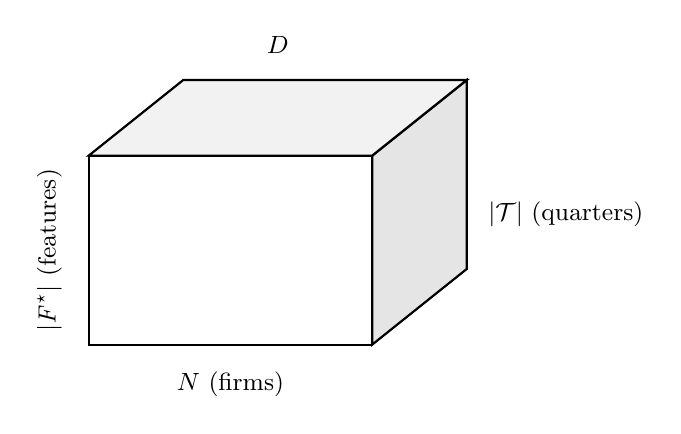
\begin{tikzpicture}[scale=1.0, every node/.style={font=\small}]
	% Design tensor cube, drawn in the same style as the model figures
	\draw[thick, fill=white] (0,0,0) -- (3.6,0,0) -- (3.6,2.4,0) -- (0,2.4,0) -- cycle;
	\draw[thick, fill=gray!20] (3.6,0,0) -- (4.8,0.96,0) -- (4.8,3.36,0) -- (3.6,2.4,0) -- cycle;
	\draw[thick, fill=gray!10] (0,2.4,0) -- (3.6,2.4,0) -- (4.8,3.36,0) -- (1.2,3.36,0) -- cycle;
	\node at (1.8,-0.5,0) {$N$ (firms)};
	\node[rotate=90] at (-0.5,1.2,0) {$|\mathit{F}^\star|$ (features)};
	\node[anchor=west] at (4.95,1.65,0) {$|\mathcal{T}|$ (quarters)};
	\node at (2.4,3.8,0) {$\mathbfcal{D}$};
	\end{tikzpicture}
	\caption[Schematic of a third-order market fundamentals design tensor.]{Schematic of a third-order market fundamentals design tensor.}
	\label{Fig:Design_Tensor_Fund}
\end{figure}

To characterize the structural complexity of $\mathbfcal{D}$ and inform the construction of MFI, we begin by applying a polyadic decomposition as follows:
\begin{equation}
	\mathbfcal{D} \approx \widehat{\mathbfcal{D}} = \sum_{r=1}^{R} \mathbf{s}_r \circ \mathbf{f}_r \circ \mathbf{t}_r,
\end{equation}
where $\mathbf{s}_r \in \mathbb{R}^N$, $\mathbf{f}_r \in \mathbb{R}^{|\mathit{F}^\star|}$, and $\mathbf{t}_r \in \mathbb{R}^{|\mathcal{T}|}$ denote the $r$th rank-one component. As shown in Figure~\ref{fig:Error_Polyadic}, the relative error of approximation decays slowly in $R$: on the order of one hundred rank-one terms are required before the observed-entry error approaches the $5\%$ level. Thus $\mathbfcal{D}$ is not well approximated by a small number of additive rank-one components, suggesting that the interactions among stocks, fundamentals, and time exhibit non-separable and highly multiway structure.

\begin{figure}[!htbp]
	\centering
	\includegraphics[scale=0.25,width=\linewidth]{./Figures/Fundamentals/Relative_Error.pdf}
	\caption[Plot of the relative error of polyadic decomposition for market fundamentals design tensor.]{Plot of the relative error of polyadic decomposition of ${\mathbfcal{D}}$ for different values of $R$.}	
	\label{fig:Error_Polyadic}
\end{figure}

Motivated by this observation, we instead employ Tucker decomposition, which generalizes matrix SVD to higher-order tensors by introducing a core tensor to capture multiway interactions. Specifically, we write
\begin{equation}
	\mathbfcal{D} \approx \widehat{\mathbfcal{D}} = \mathbfcal{H} \times_1 \mathbf{S} \times_2 \mathbf{F} \times_3 \mathbf{T},
\end{equation}
where $\mathbfcal{H} \in \mathbb{R}^{R_1 \times R_2 \times R_3}$ is the core tensor, and $\mathbf{S} \in \mathbb{R}^{N \times R_1}$, $\mathbf{F} \in \mathbb{R}^{|\mathit{F}^\star| \times R_2}$, and $\mathbf{T} \in \mathbb{R}^{|\mathcal{T}| \times R_3}$ are the factor matrices. The multilinear rank vector is defined as $\mathbf{R} = [R_1, R_2, R_3]^\intercal$. The Tucker decomposition fitted on observed entries only is obtained by solving the observed-entry optimization problem
\begin{equation}
	\label{Eq:Tucker}
	\min_{\mathbfcal{H}, \mathbf{S}, \mathbf{F}, \mathbf{T}} \left\| \mathbf{M} \odot \left(\mathbfcal{D} - \mathbfcal{H} \times_1 \mathbf{S} \times_2 \mathbf{F} \times_3 \mathbf{T}\right) \right\|_F,
\end{equation}
where $\mathbf{M}$ is the binary observation mask and $\odot$ denotes elementwise multiplication.

To preserve economic interpretability, we set $R_1$ equal to the number of observed GICS industry codes in the expanded sample and retain the full feature dimension in the second mode. This yields $R_1=67$ and $R_2=40$. We then fix $R_3=20$ to summarize the dominant temporal modes and evaluate the observed-entry relative approximation error defined by
\begin{equation}
	\label{rel_error}
	\mathrm{rel}_{\mathrm{error}} = \frac{\left\| \mathbf{M} \odot \left(\mathbfcal{D} - \widehat{\mathbfcal{D}}\right) \right\|_F}{\left\| \mathbf{M} \odot \mathbfcal{D} \right\|_F}.
\end{equation}

Rather than minimizing this error to the lowest achievable level, we intentionally select a moderate value of $R_3$ that filters out noise and captures only the most persistent components. Based on our empirical evaluation, we use the multilinear rank vector $[67,40,20]$, which yields an observed-entry relative approximation error of $5.45\%$.

Supplementary stability checks support the construction choice. Using the saved v2 time-factor matrix, replacing the mean-absolute aggregation in Definition~1 with an RMS aggregation gives a highly correlated index ($\rho=0.968$); a single-factor version is less stable ($\rho=0.581$), which supports aggregating across all temporal factors rather than selecting one component. Nearby rank/normalization checks remain close to the baseline MFI (minimum correlation $0.938$, with a no-RMS $[67,20,20]$ variant at $\rho=0.996$). An initialization audit at rank $[67,20,20]$ shows that SVD initialization reaches an observed-entry error near $5.5\%$ across iteration budgets, whereas random starts remain far above this error under the same budgets; accordingly, the reported MFI uses the SVD-initialized Tucker solution.

The temporal factor matrix $\mathbf{T}$ now contains $R_3$ latent time series of length $|\mathcal{T}|$. Each column captures a distinct latent mode of variation in the temporal dimension of the tensor. To aggregate these into a single index, we define the Market Fundamentals Index by taking the average magnitude across the $R_3$ components at each time $t$, whose formal definition is provided below.\newline

\begin{definition}[MFI]
	Let $\mathbfcal{D}$ be a third-order tensor of market fundamentals smoothed via Tucker decomposition as $\widehat{\mathbfcal{D}} = \mathbfcal{H} \times_1 \mathbf{S} \times_2 \mathbf{F} \times_3 \mathbf{T}$, with $\mathbf{T} \in \mathbb{R}^{|\mathcal{T}| \times R_3}$. The Market Fundamentals Index (MFI) is defined by
	\begin{equation}
		\mathrm{MFI}(t) := \frac{1}{R_3} \sum_{k=1}^{R_3} \left| \mathbf{T}_{t k} \right|,
	\end{equation}
	for $t = 1, \ldots, |\mathcal{T}|$.\newline
\end{definition}

The absolute value ensures that phase shifts or sign reversals do not cancel signal strength, and the averaging operation yields a smoothed, aggregate representation of the total volatility embedded in the fundamentals. As in the case of $\mathrm{FCIX}_t$, we denote the time series realization of this statistic by $\mathrm{MFI}_t$.

Figure~\ref{fig:QFCIX_MFI} displays the quarterly realizations of MFI from January 1990 through December 2024. The time series reveals distinct structural episodes, marked by substantial shifts in the volatility of firm-level fundamentals. The index rises gradually through the 1990s from a low and stable base, with a first pronounced local peak around the 2001 recession and dot-com unwind. The most elevated readings of the sample occur in 2006--2009: the index spikes sharply in late 2006 and remains elevated throughout the 2007--2009 financial crisis, reflecting heightened dispersion and instability in accounting fundamentals consistent with widespread balance sheet stress across sectors.

\begin{figure}[!htbp]
	\centering
	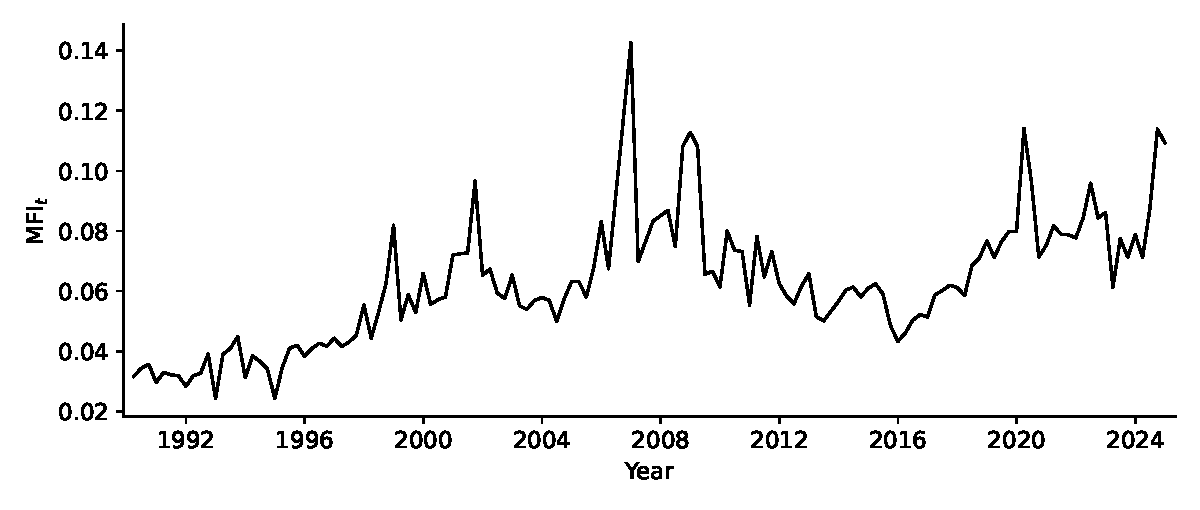
\includegraphics[width=0.95\linewidth]{./Figures/Fig_QMFI_v2}
	\caption[Quarterly $\mathrm{MFI}$.]{Plot of the quarterly  $\mathrm{MFI}$ over the period January 1990--December 2024.}
	\label{fig:QFCIX_MFI}
\end{figure}

Post-crisis, the MFI declines steadily, reaching its calmest levels around 2015-2016, where it enters a low-volatility regime with relatively minor fluctuations. An upward drift is again visible beginning in 2017-2018, culminating in a sharp spike in the first quarter of 2020 at the onset of the pandemic, and the index climbs once more toward the end of the sample in 2024. These patterns suggest that MFI effectively captures systemic dislocations in fundamental data and exhibits temporal alignment with major financial crises. The dynamics of this index and its potential predictive content are further explored in subsequent empirical tests.









%%%%%%%%%%%%%%%%%%%%%%%%%%%%%%%%%%%%%%%%%%%%%%%%%%%%%%%%%%%%%%%%%%%%%%%%%%%%%%%%%%%%%%%%%%%%%%%%%%%%%%%%%%%%%%%%%%%%%%%%%%%%%%%%%%%%%%%%



\FloatBarrier
\section{Statistical Dependence Between MFI and FCIX}
\label{Section:MFI_FCIX}

We now examine the empirical relationship between the MFI and the FCIX, with the goal of determining whether their co-movement reflects genuine statistical dependence. Because the MFI aggregates time-factor intensity in the fundamentals tensor, dependence on FCIX would mean that a fundamentals-side summary of dispersion co-moves with a price-based summary of market chaos---evidence that fundamentals dispersion and market volatility move together, revisited at the firm level in later sections.

We begin by computing the sample cross-correlation between the quarterly time series $\{\mathrm{MFI}_t\}$ and $\{\mathrm{FCIX}_t\}$ over a range of lags. Figure~\ref{Fig:Cross_Corr_Quarterly} illustrates the resulting correlation coefficients from $-10$ to $+10$ quarters. The strongest association is contemporaneous, with a peak correlation of approximately $0.32$ at lag zero, indicating a moderate near-term alignment between price-based volatility and variation in accounting fundamentals.

\begin{figure}[!htbp]
	\centering
	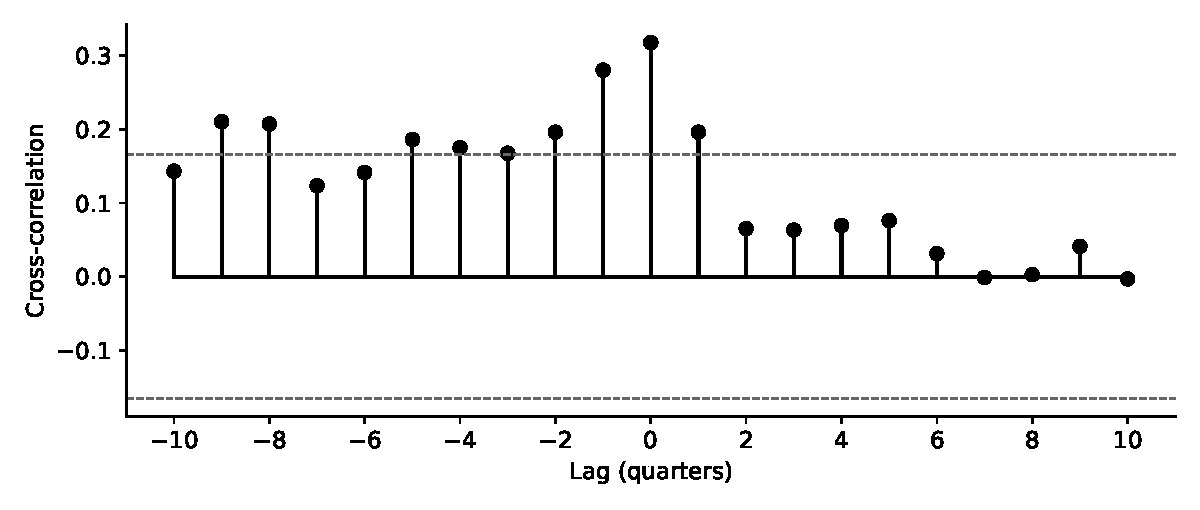
\includegraphics[width=0.95\linewidth]{./Figures/Fig_Cross_Corr_Quarters_v2.pdf}
	\caption[Cross-correlation of quarterly $\mathrm{FCIX}_t$ and $\mathrm{MFI}_t$.]{Sample cross-correlation between quarterly $\mathrm{FCIX}_t$ and $\mathrm{MFI}_t$ over the period January 1990--December 2024.}
	\label{Fig:Cross_Corr_Quarterly}
\end{figure}

While correlation provides a preliminary indication of synchrony, it is limited to capturing linear dependence and cannot rule out the possibility of spurious alignment. To test for general dependence, including nonlinear and higher-order structures, we employ a nonparametric framework based on empirical distribution comparisons. Specifically, we adopt the consistent testing methodology proposed in \citep{gretton2008nonparametric, gretton10a}, which compares the joint empirical distribution with the product of its marginals using two divergence-based test statistics.

Let $\{(\mathrm{FCIX}_t, \mathrm{MFI}_t)\}_{t=1}^{n}$ be a sequence of i.i.d. observations drawn from an unknown joint distribution $\mathbb{G}_{\mathrm{FCIX}, \mathrm{MFI}}$. Denote the corresponding marginal distributions by $\mathbb{G}_{\mathrm{FCIX}}$ and $\mathbb{G}_{\mathrm{MFI}}$. The null hypothesis of independence is expressed as:
\begin{equation*}
	\mathrm{H}_0^{\mathtt{INDP}}: \quad \mathbb{G}_{\mathrm{FCIX}, \mathrm{MFI}} = \mathbb{G}_{\mathrm{FCIX}} \times \mathbb{G}_{\mathrm{MFI}}.
\end{equation*}

Let $\mathcal{P}_n = \{A_{n,1}, \dots, A_{n,m_n}\}$ and $\mathcal{Q}_n = \{B_{n,1}, \dots, B_{n,m_n'}\}$ denote measurable partitions of $\mathbb{R}_{\geq 0}$, constructed to discretize the support of the empirical distributions. The first test statistic is based on the $L_1$ distance between the joint and product measures:
\begin{equation}
	\label{Eq:L_1_statistic}
	L_n := \sum_{A \in \mathcal{P}_n} \sum_{B \in \mathcal{Q}_n} \left| \mathbb{G}_{n,\mathrm{FCIX},\mathrm{MFI}}(A \times B) - \mathbb{G}_{n,\mathrm{FCIX}}(A)\, \mathbb{G}_{n,\mathrm{MFI}}(B) \right|.
\end{equation}

The empirical probabilities are defined by:
\begin{align}
	\mathbb{G}_{n,\mathrm{FCIX},\mathrm{MFI}}(A \times B) &:= \frac{1}{n} \sum_{t=1}^{n} \mathbb{I}[(\mathrm{FCIX}_t, \mathrm{MFI}_t) \in A \times B], \\
	\mathbb{G}_{n,\mathrm{FCIX}}(A) &:= \frac{1}{n} \sum_{t=1}^{n} \mathbb{I}[\mathrm{FCIX}_t \in A], \\
	\mathbb{G}_{n,\mathrm{MFI}}(B) &:= \frac{1}{n} \sum_{t=1}^{n} \mathbb{I}[\mathrm{MFI}_t \in B].
\end{align}

As an alternative, we compute a log-likelihood divergence statistic, which measures the Kullback--Leibler distance between the empirical joint and product-marginal distributions:
\begin{equation}
	\label{Eq:log_L_statistic}
	I_n := \sum_{A \in \mathcal{P}_n} \sum_{B \in \mathcal{Q}_n} \mathbb{G}_{n,\mathrm{FCIX},\mathrm{MFI}}(A \times B) \log \left( \frac{\mathbb{G}_{n,\mathrm{FCIX},\mathrm{MFI}}(A \times B)}{\mathbb{G}_{n,\mathrm{FCIX}}(A)\, \mathbb{G}_{n,\mathrm{MFI}}(B)} \right).
\end{equation}

Under the null hypothesis of independence, both $L_n$ and $I_n$ converge in distribution, and critical values can be approximated either via permutation or using asymptotic theory.

Table~\ref{Independence_Test} reports the results of both tests applied to $\{\mathrm{FCIX}_t\}_{t=1}^{140}$ and $\{\mathrm{MFI}_t\}_{t=1}^{140}$, using $m_n = m_n' = 6$ equal-frequency discretization bins per dimension. Critical thresholds are obtained from 10,000 random permutations of the paired quarterly series. As a serial-dependence check, we also repeat the null simulation using circular block permutations of the MFI series with four- and eight-quarter block lengths.

\begin{table}[!htbp]
	\centering
	\caption{Results of independence tests between quarterly $\mathrm{FCIX}_t$ and $\mathrm{MFI}_t$.}
	\label{Independence_Test}
	\begin{tabular}{lcc}
		\toprule
		& $L_1$-based & Log-likelihood \\
		\midrule
		Test statistic & 0.546 & 0.237 \\
		\addlinespace
		\textbf{Critical thresholds} & & \\
		\quad 1\% level   & 0.459 & 0.174 \\
		\quad 5\% level   & 0.421 & 0.148 \\
		\quad 10\% level  & 0.403 & 0.136 \\
		\addlinespace
		\textbf{Block-permutation $p$-values} & & \\
		\quad 4-quarter blocks & 0.003 & 0.006 \\
		\quad 8-quarter blocks & 0.025 & 0.043 \\
		\bottomrule
	\end{tabular}
\end{table}

Both test statistics exceed their respective iid-permutation critical values at the $1\%$ significance level, leading to the rejection of the null hypothesis $\mathrm{H}_0^{\mathtt{INDP}}$. The block-permutation check weakens the rejection, as expected for persistent quarterly series, but still rejects at conventional levels (1\% for four-quarter blocks, 5\% for eight-quarter blocks). Thus $\mathrm{FCIX}_t$ and $\mathrm{MFI}_t$ are dependent: price-based market volatility and structural shifts in accounting fundamentals are jointly distributed. We read this as evidence that the low-rank fundamentals representation carries a volatility-like factor, not as a trading claim. The next sections ask whether that structure is also useful for forecasting firm-level fundamentals, and whether markets price its forecast \emph{magnitude} (the vol channel) or its forecast \emph{errors} (the directional channel).




%%%%%%%%%%%%%%%%%%%%%%%%%%%%%%%%%%%%%%%%%%%%%%%%%%%%%%%%%%%%%%%%%%%%%%%%%%%%%%%%%%%%%%%%%%%%%%%%%%%%%%%%%%%%%%%%%%%%%%%%%%%%%%%%%%%%%%%%


\FloatBarrier
\section{Predictive Modeling for Fundamentals}
\label{Section:Predictive_Fundamentals}

Having established the MFI as a summary of cross-sectional dispersion in fundamentals and demonstrated its statistical dependence with FCIX, we now ask whether the same tensor structure contains predictive information for next-quarter accounting values---the supervised counterpart to the unsupervised index. The task is to forecast a firm-by-feature target matrix using the preceding $L$ quarters of fundamentals, with $L \in \{2,4\}$ corresponding to 6-month and 1-year lookbacks. Methodologically, this places us in the tensor-on-tensor regression literature \citep{zhou2013tensor, hoff2015multilinear, lock2018tensor}: rather than fitting a separate time-series model per accounting line item, a single low-rank multilinear map is estimated jointly across firms, features, and lags, so that predictive strength can be borrowed across the cross-section and across related line items. To our knowledge, supervised low-rank tensor regression has not previously been applied to forecasting the full joint panel of firm fundamentals.

Our design philosophy throughout this and the following sections is deliberately conservative. Model architectures and hyperparameters are selected once on a small 50-firm development set and then frozen. All later evaluations---the calendar holdout, the transfer to more firms, and the economic tests---reuse those frozen setups with no further tuning. For each economic test we state the signal, target, controls, and success criterion before looking at the results, and we report failures as well as successes.

The empirical work uses three deliberately distinct data vintages. The MFI/FCIX comparison uses fundamentals from 1990Q1--2024Q4 because the FCIX benchmark ends in 2024Q4; the prediction universe is selected using a fixed 2024Q4 market-cap snapshot; and the predictive and economic holdouts extend the fundamentals panel through 2026Q2, with the calendar-fixed training boundary unchanged.

\subsection{Tensor construction and imputation}
\label{Section:Tensor_Imputation}

From the 40 fundamental features identified in Section~\ref{Section:Feature_Selection}, we construct a quarterly predictive panel using the cleaned Compustat extract. Year-to-date cash-flow fields are converted to quarterly flows by within-fiscal-year differencing, while genuinely quarterly and trailing-twelve-month fields are retained as reported. The \emph{development} set on which all hyperparameters are tuned consists of the top $N=50$ firms by Compustat market value (`mkvaltq') at 2024Q4, a reproducible large-cap set that keeps the search computationally tractable; Section~\ref{Section:Transfer_499} refits the same frozen models on firms selected from the top $499$. We observe the development firms over 2005Q1--2024Q4, snapping report dates to a strict quarterly grid and keeping the last report per firm-quarter. This produces a raw tensor with shape $50 \times 40 \times 80$ and observed-entry density approximately $90.3\%$. Each feature is transformed by the log-modulus map
\begin{equation}
\phi(x) = \mathrm{sgn}(x)\log(1 + |x|),
\end{equation}
which stabilizes scale while preserving sign information. The resulting raw tensor is $\mathbfcal{X} \in \mathbb{R}^{N \times F \times T}$.

For each time index $t$, we form an input window and target:
\begin{equation}
\mathbfcal{X}_t = \mathbfcal{X}_{:,:,t:t+L-1} \in \mathbb{R}^{N \times F \times L},
\qquad
\mathbf{Y}_t = \mathbfcal{X}_{:,:,t+L} \in \mathbb{R}^{N \times F},
\end{equation}
with observation masks $\mathbfcal{M}_t$ and $\mathbf{M}_t$ for the input and target, respectively. Stacking across all valid time indices yields a four-dimensional input tensor $\mathbfcal{X}_{\mathrm{all}} \in \mathbb{R}^{T' \times N \times F \times L}$ and a three-dimensional target $\mathbfcal{Y}_{\mathrm{all}} \in \mathbb{R}^{T' \times N \times F}$.

Missing entries inside each input window are imputed with a Tucker decomposition fitted only on observed entries,
\begin{equation}
\min_{\mathbfcal{H}_t,\mathbf{A}_t,\mathbf{B}_t,\mathbf{C}_t}
\left\| \mathbfcal{M}_t \odot \left(\mathbfcal{X}_t -
\mathbfcal{H}_t \times_1 \mathbf{A}_t \times_2 \mathbf{B}_t \times_3 \mathbf{C}_t \right) \right\|_F^2,
\end{equation}
where $\mathbfcal{M}_t$ restricts the objective to observed entries. The fitted Tucker tensor is used only to fill missing entries; observed accounting values are preserved exactly in the covariate tensor passed to the regression step. This distinction is important because the imputer is intended to complete sparse fundamentals, not to smooth or denoise reported values.

The Tucker ranks are selected by a held-out-entry validation procedure. For each rolling window, we hide 10\% of observed entries, stratified by feature, fit the Tucker model on the remaining observed entries, and score relative Frobenius error only on the hidden entries. The time-mode rank is fixed at $L$, and the firm- and feature-mode ranks are swept over a small grid. Among configurations within one standard error of the best mean holdout error, we retain the most parsimonious choice (smallest product of firm- and feature-mode ranks). This one-standard-error rule selects ranks $(2,2,2)$ for $L=2$---where the absolute CV minimum was $(3,3,2)$ but $(2,2,2)$ is statistically tied and smaller---and $(4,4,4)$ for $L=4$, which is simultaneously the CV minimum and the one-standard-error pick. The final imputation step uses SVD initialization, a maximum of 100 iterations, and tolerance $10^{-5}$. Figure~\ref{Fig:Tucker_Imputation} illustrates the decomposition structure. We compute an observed-only RMS scale for each window,
\begin{equation}
r_t = \sqrt{\frac{1}{|\Omega_t|}\sum_{(i,j,k)\in\Omega_t} x_{ijk}^2},
\end{equation}
where $\Omega_t$ is the set of observed entries in $\mathbfcal{X}_t$. We evaluate two input-scaling variants: an unscaled covariate tensor in which missing entries are imputed in original units and observed entries remain unchanged (denoted \textsc{Unscaled}), and an RMS-normalized covariate tensor in which the completed input window is divided by $r_t$ (denoted \textsc{Normalized}).

\begin{figure}[!htbp]
\centering
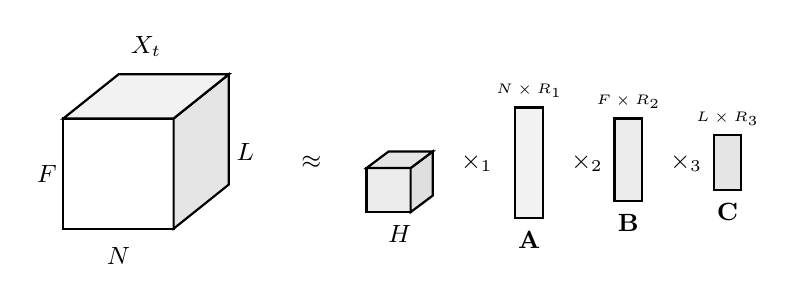
\begin{tikzpicture}[scale=0.7, every node/.style={font=\small}]
% Input tensor (3D cube)
\begin{scope}[shift={(0,0)}]
  \draw[thick, fill=white] (0,0,0) -- (2,0,0) -- (2,2,0) -- (0,2,0) -- cycle;
  \draw[thick, fill=gray!20] (2,0,0) -- (3,0.8,0) -- (3,2.8,0) -- (2,2,0) -- cycle;
  \draw[thick, fill=gray!10] (0,2,0) -- (2,2,0) -- (3,2.8,0) -- (1,2.8,0) -- cycle;
  \node at (1,-0.5,0) {$N$};
  \node at (3.3,1.4,0) {$L$};
  \node at (-0.3,1,0) {$F$};
  \node at (1.5,3.3,0) {$\mathbfcal{X}_t$};
\end{scope}

\node at (4.5,1.2) {$\approx$};

% Core tensor (smaller cube)
\begin{scope}[shift={(5.5,0.3)}]
  \draw[thick, fill=gray!15] (0,0,0) -- (0.8,0,0) -- (0.8,0.8,0) -- (0,0.8,0) -- cycle;
  \draw[thick, fill=gray!25] (0.8,0,0) -- (1.2,0.3,0) -- (1.2,1.1,0) -- (0.8,0.8,0) -- cycle;
  \draw[thick, fill=gray!20] (0,0.8,0) -- (0.8,0.8,0) -- (1.2,1.1,0) -- (0.4,1.1,0) -- cycle;
  \node at (0.6,-0.4,0) {$\mathbfcal{H}$};
\end{scope}

\node at (7.5,1.2) {$\times_1$};

% Factor A
\begin{scope}[shift={(8.2,0.2)}]
  \draw[thick, fill=gray!10] (0,0) rectangle (0.5,2);
  \node at (0.25,-0.4) {$\mathbf{A}$};
  \node at (0.25,2.3) {\tiny $N \times R_1$};
\end{scope}

\node at (9.5,1.2) {$\times_2$};

% Factor B
\begin{scope}[shift={(10,0.5)}]
  \draw[thick, fill=gray!15] (0,0) rectangle (0.5,1.5);
  \node at (0.25,-0.4) {$\mathbf{B}$};
  \node at (0.25,1.8) {\tiny $F \times R_2$};
\end{scope}

\node at (11.3,1.2) {$\times_3$};

% Factor C
\begin{scope}[shift={(11.8,0.7)}]
  \draw[thick, fill=gray!20] (0,0) rectangle (0.5,1);
  \node at (0.25,-0.4) {$\mathbf{C}$};
  \node at (0.25,1.3) {\tiny $L \times R_3$};
\end{scope}
\end{tikzpicture}
\caption{Tucker imputation for sparse fundamentals (fit on observed entries only). To resolve missing entries without discarding sparse features, the incomplete input tensor $\mathbfcal{X}_t \in \mathbb{R}^{N \times F \times L}$ is approximated by a dense core tensor $\mathbfcal{H} \in \mathbb{R}^{R_1 \times R_2 \times L}$ contracted with orthogonal factor matrices $\mathbf{A}$, $\mathbf{B}$, and $\mathbf{C}$ along each respective mode. The decomposition is fitted on observed entries only; observed values are preserved exactly, and only missing cells are filled from the low-rank reconstruction. The validated ranks are $(R_1,R_2,L)=(2,2,2)$ for the two-quarter lookback and $(4,4,4)$ for the four-quarter lookback.}
\label{Fig:Tucker_Imputation}
\end{figure}

\subsection{Low-rank CP regression as a booster}
\label{Section:CP_Structured}

The estimator is organized as a \emph{baseline-plus-booster} stack: a simple, well-understood baseline predictor absorbs the level and persistence of each firm--feature series, and a low-rank CP tensor regression is fitted to the baseline's forecast \emph{residuals}, capturing whatever cross-firm and cross-feature structure the baseline cannot represent. This architecture answers the question that matters for our purposes: does the multilinear structure add predictive information \emph{beyond} what a strong conventional model already delivers? We instantiate the stack with two baselines of increasing strength.

Throughout the prediction section, \emph{firm--feature fixed effects} (FE) means one constant per firm~$i$ and Compustat feature~$j$: the mean of observed training-window values of that series. It is \emph{not} a firm-only fixed effect, a time fixed effect, or a jointly estimated LSDV / panel FE regression; it is the classical within transform applied to the firm--feature panel, computed from training windows only and restored at prediction time.

\textit{FE baseline cell.} The first baseline sets $\widehat{\mathbf{B}}_t = \boldsymbol{\mu}$ with
\begin{equation}
\mu_{ij} = \frac{\sum_{t} m_{tij}\, y_{tij}}{\sum_{t} m_{tij} + \varepsilon},
\end{equation}
where $m_{tij}$ is the observation indicator and $\varepsilon = 10^{-8}$ prevents division by zero. Equivalently, the CP booster is trained on demeaned targets $y_{tij}-\mu_{ij}$ and the same $\mu_{ij}$ is added back in the ensemble forecast~\eqref{Eq:Ensemble}.

\textit{Ridge-booster cell.} The second baseline is the full per-feature ridge regression described in Section~\ref{Section:Baseline_Eval}---the competitive linear benchmark, which itself includes the same firm--feature FE as an additive level (Section~\ref{Section:Baseline_Eval}). Here the CP tensor is trained on the ridge model's \emph{out-of-fold} residuals: within each training set, an inner three-fold time-series split produces ridge predictions for every window from models that never saw that window. Windows without valid out-of-fold coverage are excluded from CP training rather than back-filled. This out-of-fold discipline prevents the booster from learning the baseline's in-sample optimism, and at prediction time the baseline is refitted on the full training set.

\textit{Residual target (both cells).} In either cell, write $e_{tij} = y_{tij} - \widehat{B}_{tij}$ for the baseline residual ($\widehat{B}_{tij}=\mu_{ij}$ in the FE cell, or the ridge OOF forecast in the ridge cell). The CP does \emph{not} fit levels: it fits a scaled version of $e$. Critically, this residual-target scaling is separate from the Unscaled/Normalized choice for the \emph{input} tensor $\mathbfcal{X}_t$ in Section~\ref{Section:Tensor_Imputation} (division by the window RMS $r_t$). On the residual side, two optional switches are applied in order. First, an optional per-feature scale equalizes line-item magnitudes,
\begin{equation}
\sigma_j = \sqrt{\frac{\sum_{t,i} m_{tij}\, e_{tij}^2}{\sum_{t,i} m_{tij}+\varepsilon}},
\qquad
\tilde{e}_{tij} = m_{tij}\,\frac{e_{tij}}{\sigma_j}
\end{equation}
(with $\sigma_j\equiv 1$ if the switch is off). Second, an optional global residual RMS,
\begin{equation}
s = \sqrt{\frac{1}{|\Omega|}\sum_{(t,i,j)\in\Omega}\tilde{e}_{tij}^2},
\qquad
\tilde{y}_{tij} = \frac{\tilde{e}_{tij}}{s},
\end{equation}
where $\Omega=\{(t,i,j):m_{tij}=1\}$ (with $s\equiv 1$ if the switch is off), yields the CP training target; missing entries are zero-filled. A third binary switch optionally rescales each input feature of $\mathbfcal{X}_t$ by its own training RMS; this is distinct from both $r_t$ and $(\sigma_j,s)$. The four frozen setups keep per-feature target scaling on and per-feature input scaling off; global residual RMS is on in three of four setups. Predictions undo the residual scales and remix with the baseline:
\begin{equation}
\label{Eq:Ensemble}
\widehat{y}_{tij} \;=\; \widehat{B}_{tij} \;+\; \gamma \cdot s \cdot \sigma_j \cdot \langle \mathbfcal{X}_t, \mathbfcal{W} \rangle_{ij},
\end{equation}
where $\gamma\geq 0$ is a tuned mixing weight.

In both cells, the residual map is a low-rank CANDECOMP/PARAFAC (CP) tensor regression. The coefficient tensor $\mathbfcal{W} \in \mathbb{R}^{N \times F \times L \times N \times F}$ admits the CP form
\begin{equation}
\mathbfcal{W} = \sum_{r=1}^{R} \mathbf{a}_r \circ \mathbf{b}_r \circ \mathbf{c}_r \circ \mathbf{d}_r \circ \mathbf{e}_r,
\end{equation}
where $\mathbf{a}_r \in \mathbb{R}^N$, $\mathbf{b}_r \in \mathbb{R}^F$, and $\mathbf{c}_r \in \mathbb{R}^L$ correspond to the input modes, while $\mathbf{d}_r \in \mathbb{R}^N$ and $\mathbf{e}_r \in \mathbb{R}^F$ correspond to the output modes of the $r$-th rank-one component. Figure~\ref{Fig:CP_Regression} illustrates the structure of the CP regression model.

\begin{figure}[!htbp]
\centering
\resizebox{\linewidth}{!}{%
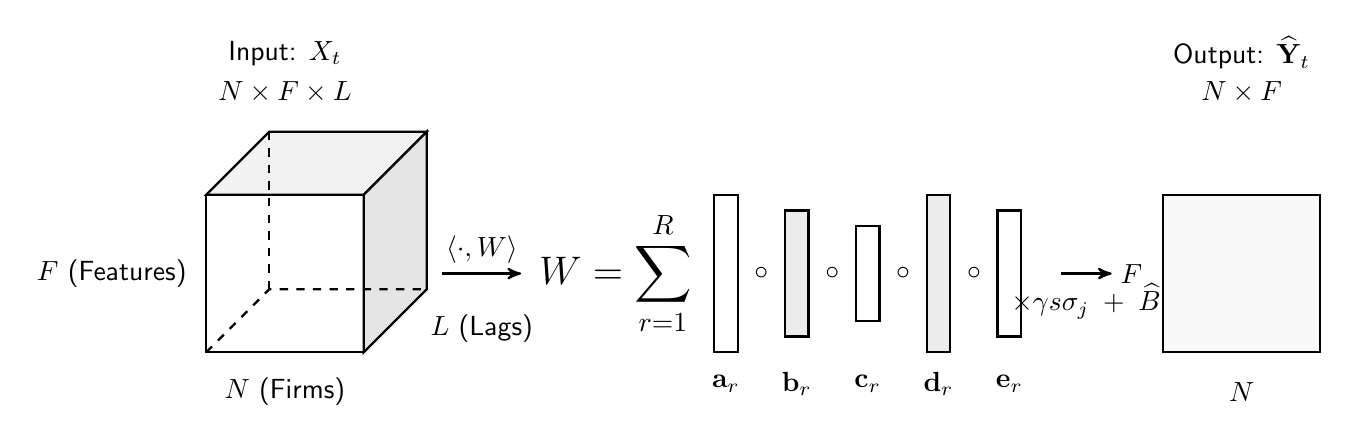
\begin{tikzpicture}[>=stealth', node distance=1.5cm, font=\sffamily]

% ===== Input tensor (3D cube) =====
\node at (1,3.8) {Input: $\mathbfcal{X}_t$};
\node at (1,3.3) {$N \times F \times L$};

\filldraw[fill=white, draw=black, thick] (0,0) rectangle (2,2);
\filldraw[fill=gray!10, draw=black, thick] (0,2) -- (0.8,2.8) -- (2.8,2.8) -- (2,2) -- cycle;
\filldraw[fill=gray!20, draw=black, thick] (2,0) -- (2.8,0.8) -- (2.8,2.8) -- (2,2) -- cycle;
\draw[dashed, thick] (0,0) -- (0.8,0.8) -- (2.8,0.8);
\draw[dashed, thick] (0.8,0.8) -- (0.8,2.8);

\node at (-1.2,1) {$F$ (Features)};
\node at (1,-0.5) {$N$ (Firms)};
\node at (3.5,0.3) {$L$ (Lags)};

% ===== Arrow: input -> contraction =====
\draw[->, thick] (3,1) -- (4,1) node[midway, above] {$\langle \cdot, \mathbfcal{W} \rangle$};

% ===== CP decomposition label =====
\node at (5.2,1) {\Large $\mathbfcal{W} = \displaystyle\sum_{r=1}^R$};

% ===== Five factor vectors (alternating white/gray) =====
\filldraw[fill=white, draw=black, thick] (6.45,0) rectangle (6.75,2);
\node at (6.6,-0.4) {$\mathbf{a}_r$};
\node at (7.05,1) {$\circ$};

\filldraw[fill=gray!15, draw=black, thick] (7.35,0.2) rectangle (7.65,1.8);
\node at (7.5,-0.4) {$\mathbf{b}_r$};
\node at (7.95,1) {$\circ$};

\filldraw[fill=white, draw=black, thick] (8.25,0.4) rectangle (8.55,1.6);
\node at (8.4,-0.4) {$\mathbf{c}_r$};
\node at (8.85,1) {$\circ$};

\filldraw[fill=gray!15, draw=black, thick] (9.15,0) rectangle (9.45,2);
\node at (9.3,-0.4) {$\mathbf{d}_r$};
\node at (9.75,1) {$\circ$};

\filldraw[fill=white, draw=black, thick] (10.05,0.2) rectangle (10.35,1.8);
\node at (10.2,-0.4) {$\mathbf{e}_r$};

% ===== Arrow: W -> output =====
\draw[->, thick] (10.85,1) -- (11.5,1) node[midway, below] {$\times \gamma s\sigma_j \;+\; \widehat{B}$};

% ===== Output matrix (N x F) =====
\node at (13.15,3.8) {Output: $\widehat{\mathbf{Y}}_t$};
\node at (13.15,3.3) {$N \times F$};

\filldraw[fill=gray!5, draw=black, thick] (12.15,0) rectangle (14.15,2);
\node at (11.75,1) {$F$};
\node at (13.15,-0.5) {$N$};

\end{tikzpicture}%
}% end resizebox
\caption{Low-rank CP tensor regression model. The 5D weight tensor $\mathbfcal{W}$ is parameterized as a sum of $R$ rank-one components. The multilinear contraction $\langle \mathbfcal{X}_t, \mathbfcal{W} \rangle$ maps the historical 3D input ($N \times F \times L$) to a 2D next-quarter residual correction ($N \times F$), which is rescaled by $\gamma s\sigma_j$ and added to the baseline forecast $\widehat{\mathbf{B}}_t$ (firm--feature FE $\mu_{ij}$, or per-feature ridge that already includes those FE).}
\label{Fig:CP_Regression}
\end{figure}

We estimate $\mathbfcal{W}$ via alternating least squares in TensorLy \citep{kossaifi2019tensorly} by regularized least squares,
\begin{equation}
\min_{\mathbfcal{W}}
\sum_t \left\| \widetilde{\mathbf{Y}}_t - \langle \mathbfcal{X}_t, \mathbfcal{W} \rangle \right\|_F^2
+ \lambda \|\mathbfcal{W}\|_F^2,
\end{equation}
where $\widetilde{\mathbf{Y}}_t$ is the zero-filled residual target $\tilde{y}_{tij}$ defined above. Because the CP regression implementation does not support fitting only on observed cells, unobserved residual targets are filled with zeros during estimation. That encoding pulls fitted residuals toward zero wherever the target was missing. Reported evaluation still scores predictions only on observed holdout entries, and the ridge benchmark uses the same zero-fill convention, so the comparison remains fair under a shared encoding. Results should therefore be read as the performance of this zero-filled estimator, not as an ideal observation-weighted CP regression.

Hyperparameters are tuned with Optuna \citep{akiba2019optuna} using a tree-structured Parzen estimator over the CP rank $R \in \{1, \ldots, 25\}$, the ridge penalty $\lambda \in [10^{-2}, 10^{5}]$ (log-uniform), the mixing weight $\gamma \in [0, 2]$, and the three binary switches above (per-feature residual scaling $\sigma_j$, global residual RMS $s$, and per-feature input scaling). The search objective is the incremental fit
\begin{equation}
\Delta R^2 \;=\; R^2\!\left(\mathbf{Y}, \widehat{\mathbf{B}} + \gamma\, \widehat{\mathrm{CP}}\right) - R^2\!\left(\mathbf{Y}, \widehat{\mathbf{B}}\right),
\end{equation}
averaged over a three-fold time-series split of the development block (the first 80\% of rolling windows), where $R^2$ is computed on all observed firm--feature--quarter cells (Section~\ref{Section:Baseline_Eval}). Scoring the \emph{extra} fit from CP over the cell's own baseline---rather than raw fit---forces the search toward genuinely complementary tensor structure. We run four parallel setups, hereafter the \emph{four frozen model setups} or \emph{cells}: firm--feature FE versus ridge as the baseline, crossed with lookback $L \in \{2,4\}$. Each cell received several thousand Optuna trials; the top-five trials per cell form a tight plateau. The single best trial in each cell is then frozen and used unchanged in every subsequent analysis in this paper.

\subsection{Ridge benchmark and evaluation protocol}
\label{Section:Baseline_Eval}

The benchmark against which the tensor must prove itself is a per-feature ridge regression on vectorized lag windows; the same model also serves as the baseline inside the ridge-booster cell of Section~\ref{Section:CP_Structured}. Both the CP and ridge models share the same firm--feature FE centering ($\mu_{ij}$ from Section~\ref{Section:CP_Structured}) and the same zero-fill convention for missing target cells; the key distinction is that each ridge model is fitted independently for a single feature with its own regularization penalty, whereas the CP tensor shares one low-rank parameterization across all features simultaneously. For each feature $j \in \{1, \ldots, F\}$, let $\mathbf{y}^{(j)} \in \mathbb{R}^{T' N}$ denote the stacked target vector and $\mathbf{X} \in \mathbb{R}^{T' N \times FL}$ the design matrix formed by flattening the lag dimension. The per-feature model is
\begin{equation}
\mathbf{y}^{(j)} = \mathbf{X} \boldsymbol{\beta}^{(j)} + \boldsymbol{\mu}^{(j)} + \boldsymbol{\epsilon}^{(j)},
\end{equation}
where $\boldsymbol{\mu}^{(j)}$ stacks the firm--feature FE $\mu_{ij}$ (constant within firm~$i$ for feature~$j$) across the time index.

Our pipeline computes those means from training windows only and models the demeaned target $y_{tij}-\mu_{ij}$ directly---the classical \emph{within transformation} for a firm--feature panel---restoring $\mu_{ij}$ at prediction time.

To make the panel structure explicit, let $\mathbf{y}_i^{(j)} \in \mathbb{R}^{T'}$ denote the time-series target for firm~$i$ and feature~$j$, and let $\mathbf{X}_i \in \mathbb{R}^{T' \times FL}$ denote the firm's design matrix. The stacked panel regression groups observations by firm:
\begin{equation} \label{eq:ridge_panel}
\begin{bmatrix}
\mathbf{y}_{1}^{(j)} \\[2pt]
\hline
\\[-8pt]
\mathbf{y}_{2}^{(j)} \\[2pt]
\hline
\\[-8pt]
\vdots \\[2pt]
\hline
\\[-8pt]
\mathbf{y}_{N}^{(j)}
\end{bmatrix}
=
\begin{bmatrix}
\mathbf{X}_{1} \\[2pt]
\hline
\\[-8pt]
\mathbf{X}_{2} \\[2pt]
\hline
\\[-8pt]
\vdots \\[2pt]
\hline
\\[-8pt]
\mathbf{X}_{N}
\end{bmatrix}
\boldsymbol{\beta}^{(j)}
+
\begin{bmatrix}
\boldsymbol{\mu}_{1}^{(j)} \\[2pt]
\hline
\\[-8pt]
\boldsymbol{\mu}_{2}^{(j)} \\[2pt]
\hline
\\[-8pt]
\vdots \\[2pt]
\hline
\\[-8pt]
\boldsymbol{\mu}_{N}^{(j)}
\end{bmatrix}
+
\begin{bmatrix}
\boldsymbol{\epsilon}_{1}^{(j)} \\[2pt]
\hline
\\[-8pt]
\boldsymbol{\epsilon}_{2}^{(j)} \\[2pt]
\hline
\\[-8pt]
\vdots \\[2pt]
\hline
\\[-8pt]
\boldsymbol{\epsilon}_{N}^{(j)}
\end{bmatrix},
\end{equation}
where $\boldsymbol{\mu}_i^{(j)} \in \mathbb{R}^{T'}$ replicates the firm--feature FE $\mu_{ij}$ across every time step. For a generic firm~$i$, the internal elements of $\mathbf{y}_i^{(j)}$ and $\mathbf{X}_i$ expand across time steps, features, and lags as:
\begin{equation} \label{eq:ridge_firm_elements}
\mathbf{y}_i^{(j)} =
\begin{bmatrix}
y_{i,\, t+1}^{(j)} \\
\vdots \\
y_{i,\, T'}^{(j)}
\end{bmatrix},
\qquad
\mathbf{X}_i =
\begin{bmatrix}
\overbrace{x_{i,\, t}^{(1)} \;\cdots\; x_{i,\, t}^{(F)}}^{\text{Lag } 1} & \cdots &
\overbrace{x_{i,\, t-L+1}^{(1)} \;\cdots\; x_{i,\, t-L+1}^{(F)}}^{\text{Lag } L} \\[4pt]
\vdots \quad \ddots \quad \vdots & \ddots & \vdots \quad \ddots \quad \vdots \\[4pt]
x_{i,\, T'\!-1}^{(1)} \;\cdots\; x_{i,\, T'\!-1}^{(F)} & \cdots &
x_{i,\, T'\!-L}^{(1)} \;\cdots\; x_{i,\, T'\!-L}^{(F)}
\end{bmatrix}.
\end{equation}

To ensure a rigorously competitive benchmark, ridge penalties are independently optimized for each feature via an inner three-fold time-series cross-validation from the candidate set $\alpha \in \{10^{-2}, 10^{-1}, 1, 10, 10^2, 10^3, 10^4\}$. This guarantees that the benchmark is optimally tuned for the specific scale and variance of every individual fundamental feature. When a feature has too few observations (below an adaptive threshold), we revert to predicting the firm-mean baseline.

Performance is evaluated using a coefficient of determination on all observed firm--feature--quarter cells,
\begin{equation}
R^2 = 1 - \frac{\sum_{t,i,j} m_{tij} (y_{tij} - \widehat{y}_{tij})^2}
{\sum_{t,i,j} m_{tij} (y_{tij} - \bar{y})^2},
\end{equation}
with $\bar{y}$ the mean of observed entries; per-feature $R^2$ values identify which fundamentals are most predictable.

\textit{Holdout fixed in calendar time.} Final evaluation uses a strict temporal split whose boundary is a calendar date, not a fraction of the sample: every window whose prediction target falls in 2021Q1 or later belongs to the test block, and no model, hyperparameter, or scaling constant sees any test-block data. Extending the panel forward only appends new test quarters; the training set is unchanged across data refreshes. On the extended panel (fundamentals through 2026Q2), this yields 62 ($L=2$) or 60 ($L=4$) training windows and 21 test windows spanning 2021Q1--2026Q2.

\subsection{Empirical results}
\label{Section:Predictive_Results}

% Numbers: prediction_new/results/v3_holdout_ext_20260629_230144/aggregate_summary.csv (rank-1 trial per cell)
Table~\ref{Tab:CP_Ridge_Results} reports test $R^2$ on observed cells for the four frozen setups on the 2021Q1--onward holdout (50-firm development set). In every setup, adding CP improves on its own baseline: by $+0.043$ to $+0.048$ over firm--feature FE alone, and---the harder comparison---by $+0.011$ to $+0.019$ over the fully tuned per-feature ridge. That ridge edge matters because ridge gets a separate, independently regularized model for every feature, while CP shares one low-rank parameterization and one global hyperparameter set across all forty. The result is robust to which Optuna trial we pick: across the top five trials in each of the four setups, all twenty holdout deltas are positive, and within the $L=2$ setups the top-five spread is below $0.002$ in $R^2$.

\begin{table}[!htbp]
\centering
\caption{Holdout results for the four frozen model setups: $R^2$ on observed cells in the calendar holdout (21 windows, 2021Q1--2026Q2; 50-firm development set). Each row is the best Optuna trial of its setup; CP is added to that setup's own baseline.}
\label{Tab:CP_Ridge_Results}
\begin{tabular}{llcccc}
\toprule
Baseline & $L$ & Baseline $R^2$ & Baseline$+$CP $R^2$ & $\Delta$ \\
\midrule
Firm--feature FE & 2 & 0.721 & \textbf{0.768} & $+0.048$ \\
Firm--feature FE & 4 & 0.722 & \textbf{0.765} & $+0.043$ \\
Ridge              & 2 & 0.764 & \textbf{0.783} & $+0.019$ \\
Ridge              & 4 & 0.767 & \textbf{0.777} & $+0.011$ \\
\bottomrule
\end{tabular}
\end{table}

% Numbers: per_feature_20260629_161824/per_feature_summary.txt (RESEARCH_LOG 2026-06-29)
Where does the gain come from? A per-feature decomposition of the CP improvement, repeated for all twenty top-five trials, shows that the gain concentrates on \emph{trending} line items. Using two train-set stationarity metrics per feature---the variance ratio $\mathrm{vr\_stat}=\mathrm{std}(\Delta x_f)/\mathrm{std}(x_f)$ of the cross-sectional mean series (low values indicate trending behavior) and a normalized trend slope---the correlation between a feature's stationarity and its CP delta is $-0.45$ to $-0.48$ (variance ratio) and $+0.44$ to $+0.50$ (trend slope) in every setup, and the most trending tercile of features gains six to twelve times more than the most stationary tercile. Figure~\ref{Fig:Booster_Stationarity} shows the ridge-baseline setups: large, trending balance-sheet and income items (total long-term debt, net sales, other assets) gain the most, while features already near-perfectly predicted by their own history (inventories, netted liabilities) gain little. The tensor's value is therefore not diffuse: it captures shared low-rank co-movement where per-feature linear-in-history models are mis-specified. Two secondary patterns fit that story: the window-level CP gain is larger when cross-sectional target dispersion is low (firms co-move), and the gain does not decay---if anything it grows slightly---across the 21-quarter test path.

\begin{figure}[!htbp]
\centering
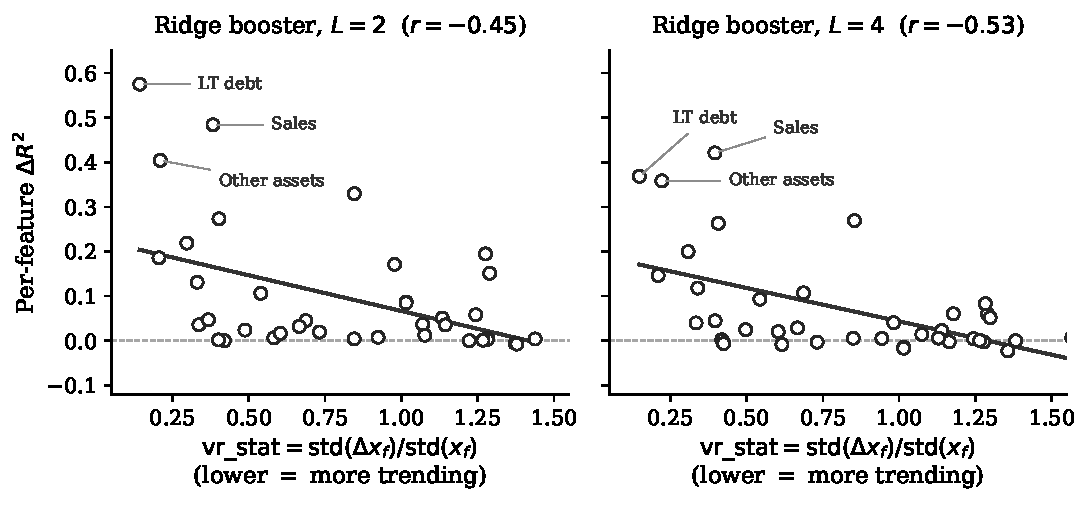
\includegraphics[width=\linewidth]{./Figures/Fig_Booster_Stationarity.pdf}
\caption{Per-feature CP improvement versus train-set stationarity. Each point is one of the 40 accounting features. The horizontal axis is $\mathrm{vr\_stat}=\mathrm{std}(\Delta x_f)/\mathrm{std}(x_f)$ (labeled on the figure; lower values are more trending). The vertical axis averages $\Delta R^2$ across the top-five Optuna trials in the frozen ridge-baseline setup. Gains concentrate on trending line items where per-feature linear history is mis-specified.}
\label{Fig:Booster_Stationarity}
\end{figure}




%%%%%%%%%%%%%%%%%%%%%%%%%%%%%%%%%%%%%%%%%%%%%%%%%%%%%%%%%%%%%%%%%%%%%%%%%%%%%%%%%%%%%%%%%%%%%%%%%%%%%%%%%%%%%%%%%%%%%%%%%%%%%%%%%%%%%%%%


\FloatBarrier
\section{Transfer to the Full Cross-Section}
\label{Section:Transfer_499}

A predictive gain established on fifty mega-caps could in principle be an artifact of that particularly well-measured corner of the market. We therefore refit all four frozen setups---hyperparameters unchanged, no re-tuning---on firms selected from the top 499 by 2024Q4 market value, using fundamentals through 2026Q2 and the same calendar holdout. One selected firm has insufficient cache coverage, so the realized panel contains 498 firms. Before estimation we required only that the CP improvement stay positive in direction: if it fell to zero or below in all four setups, that collapse would itself be the finding. Table~\ref{Tab:Transfer_499} reports the transferred holdout $R^2$ alongside the 50-firm development deltas.

% Numbers: prediction_new/results/v3_holdout_499_20260706/transfer_check_499.csv
\begin{table}[!htbp]
\centering
\caption{Transfer at frozen hyperparameters: $R^2$ on observed cells for the 498 firms that survive cache construction from the 499-firm selection set (22 test windows), compared with the 50-firm development deltas.}
\label{Tab:Transfer_499}
\begin{tabular}{llcccc}
\toprule
Baseline & $L$ & Baseline $R^2$ & $+$CP $R^2$ & $\Delta$ (499) & $\Delta$ (50) \\
\midrule
Ridge              & 2 & 0.745 & 0.759 & $+0.014$ & $+0.019$ \\
Ridge              & 4 & 0.751 & 0.762 & $+0.011$ & $+0.011$ \\
Firm--feature FE & 2 & 0.691 & 0.709 & $+0.018$ & $+0.048$ \\
Firm--feature FE & 4 & 0.693 & 0.713 & $+0.020$ & $+0.043$ \\
\bottomrule
\end{tabular}
\end{table}

The CP improvement survives in all four setups. Against ridge, the transfer delta is essentially unchanged from the 50-firm development set; against firm--feature FE alone it remains clearly positive but shrinks to roughly $40\%$ of its mega-cap size. The multilinear structure is therefore not a mega-cap artifact, though its edge over weak baselines is strongest where fundamentals are best measured---a pattern that recurs in the economic tests below.



% Computational note (Hadamard/Khatri--Rao memory-efficient ALS) omitted from
% the paper: algebraically identical to the stock solver; see code / MODEL_HISTORY.

\FloatBarrier
\section{Economic Content of Tensor Forecasts}
\label{Section:Economic_Content}

An out-of-sample $R^2$ improvement in accounting space says nothing, by itself, about economic significance. This section asks whether markets price what the forecasts contain. We separate two objects that the MFI--FCIX evidence already suggests may differ: (i)~the \emph{size} of the CP revision to the baseline---how much the tensor moves the forecast, unsigned---and (ii)~the \emph{sign} of the forecast error---whether realized fundamentals beat or miss the forecast. For each hypothesis we declare the signal, target, controls, significance criterion, and interpretation \emph{before} running the test, and we report every declared outcome, including the null ones. All tests are run separately in each of the four frozen setups; agreement across setups is treated as robustness, not as four independent replications. The size channel is already in option prices (Section~\ref{Section:Event_Study}). The sign channel is the primary economic finding---high-yield CDS tightening against an investment-grade CDS null (Section~\ref{Section:CDS})---with Section~\ref{Section:Closed_Routes} reporting the remaining equity and options diagnostics.

\subsection{Announcement event studies: returns, volatility, and option prices}
\label{Section:Event_Study}

% Numbers: v3_holdout_ext_20260629_230144/multitarget_report_ext_*.txt + FLAGGED_volrisk_report_ridge_delta_v3_L2.txt
The first battery aligns test-set forecasts with quarterly earnings announcements on the 50-firm development set (960 scored announcement events per setup over 21 test quarters). The signal declared before estimation is the \emph{size} of the CP revision: the standardized absolute difference between the ensemble and baseline predictions, available before the announcement. That object is how much the tensor revises the baseline---not the sign of the eventual error---and is the firm-level counterpart of the aggregate MFI. Outcomes include announcement-window abnormal returns and post-announcement realized and idiosyncratic volatility over the following 30 trading days, tested per feature--target pair with cross-sectional regressions and a Benjamini--Yekutieli false-discovery-rate control \citep{benjamini2001control} at $q<0.1$ over the full pair grid.

Three findings are unambiguous. First, announcement-window abnormal returns are a clean null: zero of the return-family pairs survive FDR control, in all four setups. The forecasts do not predict announcement-window price reactions in mega-caps. Second, revision size \emph{does} forecast post-announcement volatility beyond lagged realized volatility, but mainly in the ridge-baseline setups: controlling for pre-event volatility, the signal remains significant ($|t| \geq 2$) in 75 and 69 of 80 pairs in the two ridge setups, against only 13 and 6 in the two FE setups. Third, and decisive for tradeability, that volatility information is already in option prices: adding pre-event at-the-money implied volatility from OptionMetrics as a control eliminates most significant pairs in every setup (at best 29 of 80 survive, in most setups far fewer). As a tradeability check we form a straddle \emph{proxy}---not a full options backtest---equal to realized post-event volatility minus pre-event ATM IV, and long--short that residual by absolute CP revision size; means are uniformly negative or mixed, consistent with the mechanical variance risk premium rather than alpha. In short, the tensor carries a real volatility signal, consistent with MFI--FCIX dependence, but for these firms that signal is already embedded in option prices. The economically open question is therefore not revision size but error sign.

\subsection{Forecast-error signals and credit: the veer framework}
\label{Section:Veer}

% Definitions: prediction_new/veer_anomaly_experiment.py; numbers: v3_holdout_499_20260706/veer_report_*.txt
The event studies use revision \emph{size}; the richer object for pricing is the forecast \emph{error}---whether realized fundamentals beat or miss the model's prediction, and by how much. Write $e_{tij}=y_{tij}-\hat{y}_{tij}$ for the observed residual of firm $i$, feature $j$, and test quarter $t$. With a four-quarter burn-in, an expanding firm-level median $\tilde{m}_{tij}$ of past errors (pooled-feature median if the firm has fewer than two past observations) and an expanding pooled feature MAD yield the studentized surprise
\begin{equation}
\label{Eq:VeerZ}
z_{tij} \;=\; \frac{e_{tij}-\tilde{m}_{tij}}{1.4826\,\mathrm{MAD}_{tj}},
\end{equation}
using only past test quarters. Feature-level surprises are averaged within five accounting themes (leverage, earnings, investment, balance-sheet liquidity, and cash flow) to form theme-level surprise scores $\mathrm{veer}_{g,it}$ (``veers''). The \emph{cash-flow drift} used below is the three-quarter rolling mean of the cash-flow theme: firms whose cash flows have recently beaten the tensor forecast have positive drift,
\begin{equation}
\label{Eq:CashflowDrift}
\mathrm{drift}^{\mathrm{CF}}_{it} \;=\; \frac{1}{|\mathcal{W}_{it}|}\sum_{s\in\mathcal{W}_{it}} \mathrm{veer}_{\mathrm{CF},is},
\qquad
\mathcal{W}_{it}=\{s\in\{t-2,t-1,t\}:\mathrm{veer}_{\mathrm{CF},is}\text{ observed}\},
\end{equation}
requiring at least two observed quarters in the window. Analogous drifts are formed for the other themes. All signals are ex ante: they use only information available after quarter $t$'s announcement to predict outcomes over the following quarter.

On the 499-firm selection set (roughly 6{,}900 scored events per setup over 18 test quarters), we specified one primary hypothesis before evaluation: firms with persistently positive cash-flow drift should show improving credit quality. Credit quality is measured as the change in a simple Merton distance-to-default \citep{bharath2008forecasting} from two trading days before the announcement to 63 trading days after, controlling for the pre-event level and pre-trend. The test is a Fama--MacBeth regression \citep{fama1973risk} across announcement quarters. As a secondary check we report a partial rank information coefficient (rank correlation after partialling out the controls). Success requires a positive slope at one-sided $p<0.05$ in at least two of four setups.

% Numbers: veer_report_*_499.txt; PD translation: h1_pd_translation_499.csv
The hypothesis is supported; Table~\ref{Tab:H1_DD} reports the four setups. The Fama--MacBeth slope is $+0.020$ in \emph{all four setups}, with one-sided $p = 0.033$ and $0.040$ in the two FE setups, $p = 0.060$ and $0.071$ in the ridge setups, and a positive partial rank IC ($t \approx +2.1$ to $+2.6$) throughout.

\begin{table}[!htbp]
\centering
\caption{Credit test declared before estimation on the 499-firm selection set: Fama--MacBeth slope of the post-announcement change in distance-to-default on cash-flow drift, with pre-event level and pre-trend controls ($\approx$6{,}900 events per setup; declared sign positive, one-sided $p$; success bar: $p<0.05$ in $\geq 2$ of 4 setups).}
\label{Tab:H1_DD}
\begin{tabular}{llcccc}
\toprule
Baseline & $L$ & Slope & $t$ & One-sided $p$ & Partial IC $t$ \\
\midrule
Ridge              & 2 & $+0.0204$ & $+2.06$ & 0.060 & $+2.1$ \\
Ridge              & 4 & $+0.0197$ & $+1.97$ & 0.071 & $+2.2$ \\
Firm--feature FE & 2 & $+0.0202$ & $+2.28$ & 0.040 & $+2.4$ \\
Firm--feature FE & 4 & $+0.0204$ & $+2.39$ & 0.033 & $+2.6$ \\
\bottomrule
\end{tabular}
\end{table}
In economic units, a one-standard-deviation increase in cash-flow drift maps to a distance-to-default improvement of $+0.05$ to $+0.07$. Relative to the panel's distance-to-default distribution, that is a $29\%$ to $56\%$ \emph{relative} reduction in the model-implied physical default probability, larger when the firm starts with better credit quality. Absolute default probabilities in this mostly investment-grade panel are tiny, so a large relative change need not show up in traded prices; the next subsection tests that. A secondary hypothesis declared before estimation---that the joint set of veer scores helps explain post-announcement changes in implied volatility---passed formally in three of four setups but with $R^2$ increments of at most $+0.003$; we treat it as economically negligible, consistent with the option-price result above.

\subsection{Traded credit: high-yield result against an investment-grade null}
\label{Section:CDS}

% Numbers: cds_h1_translation_499.csv + cds_h1_translation_hy.csv
We next ask whether that credit information shows up in traded CDS spreads. The same cash-flow drift that improves distance-to-default in Section~\ref{Section:Veer} leaves investment-grade CDS spreads unmoved, yet predicts economically meaningful tightening in a high-yield and crossover sample. Table~\ref{Tab:CDS_IG_vs_HY} summarizes both tests: roughly $\pm 0.03$ basis points per one-standard-deviation cash-flow drift at the investment-grade median spread, against about $-6.5$ basis points per one-standard-deviation cash-flow drift at the high-yield median, with the expected negative sign in all four frozen setups.

\begin{table}[!htbp]
\centering
\caption{Comparison of CDS responses: post-announcement change in log five-year CDS on a one-standard-deviation cash-flow drift (same window and controls). Investment-grade sample: 1{,}961 events, 169 firms. High-yield sample: 900 events, 90 firms. Ranges are across the four frozen setups; bp columns are spread change per $1\sigma$ of cash-flow drift at each sample's median spread.}
\label{Tab:CDS_IG_vs_HY}
\begin{tabular}{lccc}
\toprule
Universe & Median spread & bp per $1\sigma$ CF drift & Setups (expected sign) \\
\midrule
Investment-grade CDS overlap & 56 bp & $\pm 0.03$ & flat ($|t|<0.15$) \\
High-yield / crossover & 282 bp & $-6.3$ to $-6.9$ & 4/4 ($p_{1s}<0.05$) \\
\bottomrule
\end{tabular}
\end{table}

% Universe: build_hy_universe.py; numbers: v3_holdout_hy_20260707/cds_h1_translation_hy.csv
For the high-yield sample we built a dedicated crossover and high-yield universe and declared the hypothesis before estimation. From U.S.\ five-year senior CDS reference entities in Markit, we kept issuers with median spreads of at least 150 basis points and matched them to listed CRSP/Compustat firms, yielding 113 names with a median spread of 289 basis points, against 56 in the investment-grade sample.\footnote{Matching is by normalized issuer name, with financing subsidiaries mapped to their listed parents and private or defunct entities excluded. Of 970 reference entities, 298 met the spread threshold and 128 matched, of which 113 had sufficient fundamentals coverage.} Because the universe is defined at 2024Q4, defaulted names are missing, which biases against the hypothesis. The full pipeline was re-estimated with the same frozen hyperparameters; the CP improvement stays positive in three of four setups and turns negative in the FE baseline with $L=4$, consistent with low-rank structure weakening as fundamentals become noisier down the credit spectrum. Table~\ref{Tab:HY_CDS} reports the declared Fama--MacBeth test.

\begin{table}[!htbp]
\centering
\caption{High-yield CDS test declared before estimation: Fama--MacBeth slope of the post-announcement change in log five-year CDS spread on cash-flow drift, with pre-event spread level and pre-trend controls (900 events, 90 CDS-covered firms, 13 quarters per setup; declared sign negative, one-sided $p$). The final column converts the slope to basis points of spread change per one-standard-deviation cash-flow drift, evaluated at the 282 bp sample median spread.}
\label{Tab:HY_CDS}
\begin{tabular}{llcccc}
\toprule
Baseline & $L$ & Slope & $t$ & One-sided $p$ & bp per $1\sigma$ CF drift \\
\midrule
Ridge              & 2 & $-0.0113$ & $-2.21$ & 0.024 & $-6.3$ \\
Ridge              & 4 & $-0.0151$ & $-2.74$ & 0.009 & $-6.8$ \\
Firm--feature FE & 2 & $-0.0112$ & $-2.34$ & 0.019 & $-6.9$ \\
Firm--feature FE & 4 & $-0.0104$ & $-1.96$ & 0.037 & $-6.4$ \\
\bottomrule
\end{tabular}
\end{table}

The high-yield test meets the pre-specified sign and significance bar in \emph{all four setups} (the bar was two of four). In crossover and high-yield names, a one-standard-deviation increase in cash-flow drift predicts approximately $2.3\%$ of spread tightening---about 6.5 basis points at the median spread---over the following quarter, controlling for the spread level and its pre-trend. Partial rank ICs are negative in all four setups. Given the small sample (90 firms, 13 quarters) and the correlation across setups, we count this as one supported result, not four independent ones.

We subject this CDS result to a small robustness battery, summarized in Table~\ref{Tab:HY_CDS_Robust}. The sign is stable: the cash-flow drift coefficient is negative in every setup under log-spread changes at 21-, 42-, and 63-trading-day horizons, under raw-basis-point spread changes, after one-quarter-at-a-time deletions, and within each pre-event spread tercile. Statistical strength is not uniform. The 42-day window is strongest; raw spread changes preserve the economic sign and imply larger basis-point moves but are noisier; 5\% winsorization and dropping 2022 quarters attenuate significance in some setups. The tercile split is useful: the basis-point effect is largest in the widest-spread tercile, where default risk is closest to the money.

\begin{table}[!htbp]
\centering
\caption{High-yield CDS robustness summary. Entries aggregate the four frozen setups. The sign column reports how many setups have the expected negative slope; the basis-point range is the implied effect of a one-standard-deviation cash-flow drift at the relevant median spread.}
\label{Tab:HY_CDS_Robust}
\begin{tabular}{lccc}
\toprule
Variant & Expected sign & bp range & Comment \\
\midrule
Log spread, +21td & 4/4 & $-3.9$ to $-4.4$ & shorter-window effect \\
Log spread, +42td & 4/4 & $-6.3$ to $-6.7$ & strongest t-statistics \\
Log spread, +63td & 4/4 & $-6.3$ to $-6.9$ & primary window \\
Raw spread change, +63td & 4/4 & $-12.4$ to $-14.5$ & noisier in levels \\
1\% winsorized, +63td & 4/4 & $-5.6$ to $-6.4$ & sign intact \\
5\% winsorized, +63td & 4/4 & $-4.0$ to $-5.1$ & attenuated \\
Drop 2022 quarters & 4/4 & $-5.4$ to $-6.5$ & reduced power \\
Leave-one-quarter-out & 4/4 & $-5.0$ to $-8.6$ & sign never flips \\
Widest spread tercile & 4/4 & $-11.9$ to $-18.4$ & largest economic effect \\
\bottomrule
\end{tabular}
\end{table}

% Numbers: v3_holdout_499_20260706/cds_h1_translation_499.csv
By contrast, the same specification on Markit five-year CDS matched to 169 of the 499 selection-set firms is a clean null in all four setups: slopes are indistinguishable from zero ($|t| < 0.15$), amounting to $\pm 0.03$ basis points per one-standard-deviation cash-flow drift at the sample's 56 basis-point median spread. The null is not a matching artifact: re-running the distance-to-default regression on exactly the CDS-covered subsample leaves the slope intact and slightly larger ($+0.024$ to $+0.026$, $t > 2$). The same firm-events whose model-implied credit quality improves show no movement in their traded spread. Within the investment-grade panel, the distance-to-default effect concentrates in the highest spread tercile in all four setups, which motivates the high-yield extension above rather than an investment-grade trading claim.

\subsection{Equity, options, and error-structure diagnostics}
\label{Section:Closed_Routes}

We also evaluate several non-CDS outcomes that were specified before estimation. None overturns the credit comparison in Section~\ref{Section:CDS}, and none is a second primary claim.

An options-tradeability battery was specified beforehand on the high-yield universe, using the same straddle proxy as in Section~\ref{Section:Event_Study} (long--short of realized vol minus pre-event ATM IV, sorted on absolute CP revision size). The primary criterion---a positive and bootstrap-significant long--short mean in at least two of four setups---was met exactly at the declared bar, but only in the two $L=4$ setups; the secondary criterion (per-pair significance incremental to implied volatility) failed in all four. We read this as a weak effect that appears only for the longer lookback, and we do not advance it as a second economic finding.

Cash-flow drift does \emph{not} predict forward equity returns in the 499-firm selection set (Fama--MacBeth $t < 0.8$ everywhere; tercile long--short spreads positive but insignificant). Equity tests therefore find no usable signal here for either revision size or error sign.

Forecast errors are essentially idiosyncratic: clustering firms by error co-movement recovers no sectoral structure (adjusted Rand index versus GICS below $0.04$ in every setup) and the first principal component explains under $4\%$ of error variance. The veer scores therefore behave as firm-specific news rather than as a missed common factor.

\FloatBarrier
\section{Conclusion}

This paper follows one arc from tensor structure in firm fundamentals to where markets price it. From a third-order Compustat tensor we construct the Market Fundamentals Index as a summary of cross-firm dispersion in fundamentals and show its statistical dependence on price-based chaos (FCIX)---evidence that accounting dispersion and market volatility move together. The same structure, as CP trained on residuals after ridge or firm--feature FE baselines, improves next-quarter forecasts on a 50-firm development set and, with the same frozen hyperparameters, on a wider selection set. Gains concentrate on trending line items where linear history is mis-specified.

Pricing splits by object. The \emph{size} of the CP revision predicts post-announcement volatility in mega-caps, but option-implied volatility already contains that information---the firm-level counterpart of MFI--FCIX. The \emph{sign} of forecast errors is where incorporation is uneven. Firms whose cash flows beat the tensor forecast for several quarters show improving distance-to-default, yet investment-grade CDS spreads do not move. In crossover and high-yield credit, a one-standard-deviation increase in cash-flow drift predicts about 6.5 basis points of spread tightening over the following quarter in all four frozen setups. Equity and options tests are insignificant or fragile. Markets appear to absorb the tensor's volatility content in liquid names and to price signed fundamentals residuals more slowly where default risk is material.

The analysis has candid limitations. The high-yield sample is short and defined at a fixed date, so defaulted firms are missing. The four model setups are correlated rather than independent replications. Equity and options tests find no usable signal. Because CP fills missing residual targets with zeros in training, a natural extension is observation-weighted CP estimation to see whether removing that pull toward zero changes the forecast gains. Other natural extensions include longer high-yield histories, including dead firms to remove the survival bias, and routing the veer scores to credit instruments that can be traded at scale.
%%%%%%%%%%%%%%%%%%%%%%%%%%%%%%%%%%%%%%%%%%%%%%%%%%%%%%%%%%%%%%%%%%%%%%%%%%%%%%%%%%%%%%%%%%%%%%%%%%%%%%%%%%%%%%%%%%%%%%%%%%%%%%%%%%%%%%%%




%\subsection{Block-wise Granger Causality}
%\label{Section:7_4}
%Let us first assume that the market fundamentals index is already at our disposal. Hence, we may devote the remainder of this section to discover the existence of causal relations from \textit{policy uncertainty indexes} to $\mathrm{FCIX}_t$ by further taking into account the assets' fundamentals information. To this end, we first formulate a conditional null hypothesis and then perform a \textit{$1$-step block-wise Granger causality} test to identify and characterize possible causal relations. A reason for choosing only $1$-step-ahead Granger causality tests, is due to the observation that selecting a minimal possible time-horizon size (i.e., $h=1$ or equivalently, one single quarter of the time unit) could be sufficient to capture potential changes in macroeconomic factors and assets' fundamentals that may influence the stock market trends. In addition, inspection of  \ref{Fig:Cross_Corr_Quarterly} supports our choice for the size of time-horizon, whereby it is observed that the maximum cross-correlation between $\mathrm{FCIX}_t$ and $\mathrm{MFI}_t$ occurs at $1$-lag quarter having its value to be $73.378\%$.
%
%Denote by $\mathcal{J}_{t,\mathtt{Q}}^{\mathtt{PRC}} = \mathscr{F}_{\mathrm{FCIX},t}$ the set of known information for $\mathrm{FCIX}_t$ up to a quarter of time unit $t$. Also, we will slightly abuse the notation, by using $\mathbf{F}_t$ to represent $\mathrm{FCIX}_t$. Let us now define the following quarterly multivariate time series
%\begin{equation*}
%	\mathbf{U}_t = \left( \mathrm{VIX}_t, \mathrm{MFI}_t \right)^\intercal  ,
%\end{equation*}
%and
%\begin{equation*}
%	\resizebox{1\hsize}{!}  { $\mathbf{W}_t = \left( \mathrm{EMV}_t, \mathrm{EPU}_t, \mathrm{MON}_t, \mathrm{FIS}_t, \mathrm{TAX}_t, \mathrm{GOV}_t, \mathrm{HLTH}_t, \mathrm{SEC}_t, \mathrm{ENT}_t, \mathrm{GREG}_t, \mathrm{FREG}_t, \mathrm{TRD}_t, \mathrm{CPI}_t \right)^\intercal $}  ,
%\end{equation*}
%with their respective sets of the known information represented by $ \mathscr{F}_{\mathrm{VIX},t} \bigotimes \mathscr{F}_{\mathrm{MFI},t} $, and  $$ \mathcal{J}_{t,\mathtt{Q}}^{\mathtt{NEWS}} = \bigotimes_{k=1}^K \mathscr{F}_{\mathbf{W}_{k},t}  ,$$ where $K=13$.
%
%Next, we would like to test whether the group of individual univariate components of $\mathbf{W}_t$ are not a $1$-step Granger cause of $\mathrm{FCIX}_t$, given the information on the respective components of $\mathbf{U}_t$. However, since both components of $\mathbf{U}_t$ are statistically dependent on $\mathrm{FCIX}_t$, i.e., $\mathrm{VIX}_t$ dependents through cointegration (e.g., see \ref{Section:5_2}) and $\mathrm{MFI}_t$ by implications of the independence tests executed in \ref{Section:7_3}, then possibilities of inferring spurious causalities would potentially be eliminated if these common dependencies ($\mathrm{VIX}_t$ and $\mathrm{FCIX}_t$) are \textit{conditioned out}.
%
%To this end, we express the joint distribution of the multivariate processes $(\mathbf{F}_t,\mathbf{W}_t,\mathbf{U}_t)^\intercal$ in VAR($p$) form as follows:
%\begin{equation}
%	\label{Eq:VAR_MFI}
%	\begin{pmatrix}
%		\mathbf{F}_t \\
%		\mathbf{W}_t \\
%		\mathbf{U}_t 
%	\end{pmatrix} 
%	= \nsum\limits_{k=1}^p
%	\begin{pmatrix}
%		b_{ff,k} & b_{fw,k} & b_{fu,k} \\
%		b_{wf,k} & b_{ww,k} & b_{wu,k} \\
%		b_{uf,k} & b_{uw,k} & b_{uu,k}
%	\end{pmatrix} 
%	\begin{pmatrix}
%		\mathbf{F}_{t-k} \\
%		\mathbf{W}_{t-k} \\
%		\mathbf{U}_{t-k} 
%	\end{pmatrix}
%	+
%	\begin{pmatrix}
%		{\epsilon}_{f,t} \\
%		\boldsymbol{\epsilon}_{w,t} \\
%		\boldsymbol{\epsilon}_{u,t} 
%	\end{pmatrix}  .
%\end{equation}
%Here, the residual variance-covariance matrix of the error vectors takes on a form as follows:
%\begin{equation}
%	\boldsymbol{\Sigma} = 
%	\mathrm{cov}
%	\begin{pmatrix}
%		{\epsilon}_{f,t} \\
%		\boldsymbol{\epsilon}_{w,t} \\
%		\boldsymbol{\epsilon}_{u,t} 
%	\end{pmatrix} 
%	= 
%	\begin{pmatrix}
%		{\Sigma}_{ff} & \boldsymbol{\Sigma}_{fw} & \boldsymbol{\Sigma}_{fu} \\
%		\boldsymbol{\Sigma}_{wf} & \boldsymbol{\Sigma}_{ww} & \boldsymbol{\Sigma}_{wu} \\
%		\boldsymbol{\Sigma}_{uf} & \boldsymbol{\Sigma}_{uw} & \boldsymbol{\Sigma}_{uu}
%	\end{pmatrix}  . 
%\end{equation}
%Note that that the relation given by \ref{Eq:VAR_MFI} does not involve neither the shift nor a linear trend components due to the fact that $\mathrm{FCIX}_t$ is an $I(1)$ process with no shift or linear trend, as per \ref{Section:3_2}. Subsequently, by analogy to \ref{Section:6}, we express the \textit{unrestricted} and \textit{restricted} regression models by
%\begin{equation}
%	\mathbf{F}_t = \sum\limits_{k=1}^p b_{ff,k} \mathbf{F}_{t-k} + \sum\limits_{k=1}^p b_{fw,k} \mathbf{W}_{t-k}  + \sum\limits_{k=1}^p b_{fu,k} \mathbf{U}_{t-k} + {\epsilon}_{f,t}  ,
%\end{equation}
%and
%\begin{equation}
%	\mathbf{F}_t = \sum\limits_{k=1}^p b_{ff,k}^{'} \mathbf{F}_{t-k} + \sum\limits_{k=1}^p b_{fu,k}^{'} \mathbf{U}_{t-k} + {\epsilon}_{f,t}^{'}  ,
%\end{equation}
%respectively, where the variables used for conditioning that are contained in $\mathbf{U}_t$, are present in both of the above models. 
%
%In turn, the null hypothesis on no causality is formulated as follows:
%\begin{equation*}
%	\mathrm{H}_{0,\mathtt{Q}}^{\mathtt{NEWS}} : \forall k\in\{1,2\dots,p\}, b_{wf,k} = 0  ,
%\end{equation*}
%whose corresponding alternative hypothesis is:
%\begin{equation*}
%	\mathrm{H}_{1,\mathtt{Q}}^{\mathtt{NEWS}} : \exists k\in\{1,2\dots,p\}, b_{wf,k} \neq 0  .
%\end{equation*}
%Similar to \ref{EQ:GC_Measure}, the test statistic based on the generalized variance of the regression models is utulized, which estimates the \textit{model prediction error} and is given by the following \text{log-likelihood ratio}:
%\begin{equation}
%	\label{EQ:GC_Measure_Conditional}
%	\mathrm{GC}_{\mathbf{W}_t\overset{h=1}{\nrightarrow} \mathbf{F}_t|\mathbf{U}_t} = \log \frac{|\Sigma_{ff}^{'}|}{|\Sigma_{ff}|}  \cdot
%\end{equation}
%
%\ref{Blockwise_News_Results} summarizes the results obtained for testing $\mathrm{H}_{0,\mathtt{Q}}^{\mathtt{NEWS}}$. Both $\chi^2$ and $F$ underlying distributions for the test statistics were considered. As per these results, there is no sufficient evidence to reject the null hypothesis $\mathrm{H}_{0,\mathtt{Q}}^{\mathtt{NEWS}}$ at $1\%$ level of significance using either of these test statistics. In turn, this implies that the mutual quarterly price changes of the assets are $1$-step Granger caused by news-based uncertainty indexes, given the known information sets pertaining to $\mathrm{VIX}_t$ and $\mathrm{MFI}_t$. In other words, the null hypothesis does not get rejected w.r.t. the known information set  $\mathcal{J}_{t,\mathtt{Q}}^{\mathtt{PRC}} \bigoplus \mathcal{J}_{t,\mathtt{Q}}^{\mathtt{NEWS}} | \mathscr{F}_{\mathrm{VIX},t} \bigotimes \mathscr{F}_{\mathrm{MFI},t}.$
%
%\begin{table}[ht]
%	\centering
%	\footnotesize
%	\caption{Results of Granger causality test for $\mathrm{H}_{0,\mathtt{Q}}^{\mathtt{NEWS}}$.}
%	\label{Blockwise_News_Results}
%	\begin{tabular}{lcc} 
%		\toprule
%		& $\chi^2$-test & $F$-test \\
%		\midrule
%		p-value         & 0.129   & 0.234 \\
%		Test statistics & 63.663  & 1.224 \\
%		\addlinespace
%		\textbf{Critical values} & & \\
%		\quad 1\% level  & 78.660  & 1.923 \\
%		\quad 5\% level  & 69.832  & 1.585 \\
%		\quad 10\% level & 65.422  & 1.431 \\
%		\bottomrule
%	\end{tabular}
%\end{table}
%
%	
%	Moreover, it is very important to investigate the impacts of news-based information ($\mathcal{J}_{t,\mathtt{Q}}^{\mathtt{NEWS}}$) augmented with the fundamentals' information ($\mathscr{F}_{\mathrm{MFI},t}$), on the price-generating mechanisms of the assets. As we may assume without the loss of generality that such an augmented set of information alongside the price-related sets of known information ($\mathscr{F}_{\mathrm{FCIX},t}$ and $\mathscr{F}_{\mathrm{VIX},t}$) contains all the \textit{publicly known information} about the assets. To this end, we reshape the configuration of the elements contained in the multivariate time series $\mathbf{W}_t$ and $\mathbf{U}_t$, and introduce two new time series
%	\begin{equation*}
%		\mathbf{\widetilde{U}}_t =  \mathrm{VIX}_t   ,
%	\end{equation*}
%	and
%	\begin{equation*}
%		\resizebox{1\hsize}{!}  { $\mathbf{\widetilde{W}}_t = \left( \mathrm{MFI}_t, \mathrm{EMV}_t, \mathrm{EPU}_t, \mathrm{MON}_t, \mathrm{FIS}_t, \mathrm{TAX}_t, \mathrm{GOV}_t, \mathrm{HLTH}_t, \mathrm{SEC}_t, \mathrm{ENT}_t, \mathrm{GREG}_t, \mathrm{FREG}_t, \mathrm{TRD}_t, \mathrm{CPI}_t \right)^\intercal $} ,
%	\end{equation*}
%	whose respective sets of known information are represented by $ \mathscr{F}_{\mathrm{VIX},t}  $ and $$ \mathcal{J}_{t,\mathtt{Q}}^{\mathtt{PUB}} = \left( \bigotimes_{k=2}^{K^{'}} \mathscr{F}_{\mathbf{\widetilde{W}}_{k},t} \right) \bigoplus \mathscr{F}_{\mathrm{MFI},t}  , $$ where $K{'}=14$. Thereafter, the corresponding \textit{unrestricted} and \textit{restricted} regression models are re-derived, but for this time it is to be done by substituting $\mathbf{\widetilde{U}}_t$ for $\mathbf{U}_t$ and $\mathbf{\widetilde{W}}_t$ for $\mathbf{W}_t$. Subsequently, we reformulate a null hypothesis as follows:
%	\begin{equation*}
%		\mathrm{H}_{0,\mathtt{Q}}^{\mathtt{PUB}} : \forall k\in\{1,2\dots,p\},  \tilde{b}_{\tilde{w}f,k} = 0  ,
%	\end{equation*}
%	and test it versus the following alternative:
%	\begin{equation*}
%		\mathrm{H}_{1,\mathtt{Q}}^{\mathtt{PUB}} : \exists k\in\{1,2\dots,p\},  \tilde{b}_{\tilde{w}f,k} \neq 0  .
%	\end{equation*}
%	The corresponding test statistic is further given by
%	\begin{equation}
%		\label{EQ:GC_Measure_Conditional_Pub}
%		\mathrm{GC}_{\mathbf{\widetilde{W}}_t\overset{h=1}{\nrightarrow} \mathbf{F}_t|\mathbf{\widetilde{U}}_t} = \log \frac{|\widetilde{\Sigma}_{ff}^{'}|}{|\widetilde{\Sigma}_{ff}|}  \cdot
%	\end{equation}
%	
%	
%\begin{table}[ht]
%	\centering
%	\footnotesize
%	\caption{Results of Granger causality test for $\mathrm{H}_{0,\mathtt{Q}}^{\mathtt{PUB}}$.}
%	\label{Blockwise_Public_Results}
%	\begin{tabular}{lcc} 
%		\toprule
%		& $\chi^2$-test & $F$-test \\
%		\midrule
%		p-value         & 0.014   & 0.134 \\
%		Test statistics & 98.603  & 1.409 \\
%		\addlinespace
%		\textbf{Critical values} & & \\
%		\quad 1\% level  & 100.425 & 2.072 \\
%		\quad 5\% level  & 90.531  & 1.665 \\
%		\quad 10\% level & 85.527  & 1.486 \\
%		\bottomrule
%	\end{tabular}
%\end{table}
%
%
%According to the results presented in \ref{Blockwise_Public_Results}, there is insufficient evidence to reject the null hypothesis that the market fundamentals index alongside newschapter-based uncertainty indexes do not $1$-step Granger cause $\mathrm{FCIX}_t$ at $1\%$ level of significance, i.e., the null hypothesis does not get rejected w.r.t. the known information set $\mathcal{J}_{t,\mathtt{Q}}^{\mathtt{PRC}} \bigoplus \mathcal{J}_{t,\mathtt{Q}}^{\mathtt{PUB}} | \mathscr{F}_{\mathrm{VIX},t} $. In  turn, this implies that the quarterly price changes exhibited by the mutual behavior of the assets in the stock market are $1$-step Granger caused by macroeconomic and/or policy uncertainty news as well as the fundamentals-related information. 
%
%
%
%




%%%%%%%%%%%%%%%%%%%%%%%%%%%%%%%%%%%%%%%%%%%%%%%%%%%%%%%%%%%%%%%%%%%%%%%%%%%%%%%%%%%%%%%%%%%%%%%%%%%%%%%%%%%%%%%%%%%%%%%%%%%%%%%%%%%%%%%%
%%%%%%%%%%%%%%%%%%%%%%%%%%%%%%%%%%%%%%%%%%%%%%%%%%%%%%%%%%%%%%%%%%%%%%%%%%%%%%%%%%%%%%%%%%%%%%%%%%%%%%%%%%%%%%%%%%%%%%%%%%%%%%%%%%%%%%%%
%%%%%%%%%%%%%%%%%%%%%%%%%%%%%%%%%%%%%%%%%%%%%%%%%%%%%%%%%%%%%%%%%%%%%%%%%%%%%%%%%%%%%%%%%%%%%%%%%%%%%%%%%%%%%%%%%%%%%%%%%%%%%%%%%%%%%%%%




































%%%%%%%%%%%%%%%%%%%%%%%%%%%%%%%%%%%%%%%%%%%%%%%%%%%%%%%%%%%%%%%%%%%%%%%%%%%%%%%%%%%%%%%%%%%%%%%%%%%%%%%%%%%%%%%%%%%%%%%%%%%%%%%%%%%%%%%%
%%%%%%%%%%%%%%%%%%%%%%%%%%%%%%%%%%%%%%%%%%%%%%%%%%%%%%%%%%%%%%%%%%%%%%%%%%%%%%%%%%%%%%%%%%%%%%%%%%%%%%%%%%%%%%%%%%%%%%%%%%%%%%%%%%%%%%%%
%%%%%%%%%%%%%%%%%%%%%%%%%%%%%%%%%%%%%%%%%%%%%%%%%%%%%%%%%%%%%%%%%%%%%%%%%%%%%%%%%%%%%%%%%%%%%%%%%%%%%%%%%%%%%%%%%%%%%%%%%%%%%%%%%%%%%%%%


%\section{The Efficient Market Hypothesis}
%\label{Section:8}
%In the last section of our chapter, we employ the previously developed tools and concepts and concentrate on the long-standing \textit{efficient market hypothesis} (EMH). The literature on EMH and its definition is vast and extensive; we refer the interested reader to \citep{degutis2014efficient,gabriela2015efficient,naseer2015efficient, lehmann1990fads, stein1989efficient, shi2018should}, to list a few. However, in some broad sense, EMH stipulates that market prices fully reflect all available information, further implying that the sequences of the asset price changes would behave in a more random manner in the case where the market exhibits larger degrees of efficiency, to the extent that in a completely efficient market the price changes would be completely unpredictable. 
%
%One possible approach that we follow in this section is to formulate the EMH using the notion of the financial chaos index. Note that such a possibility stems from the remark made in \ref{Section:3} where it was discussed that $\mathrm{FCIX}_t$ could potentially be considered as a consistent and robust estimator of the market volatility. Hence, we present three versions of the EMH formulated in terms of the financial chaos index which are in the same spirit as to the definitions provided in \citep{jensen1978some}. 
%
%We stress the fact that failure to reject EMH, or alternatively accept it, has few implications for efficiency of the market price formations insofar as there is insufficient existence of a thorough and explicit economic model accounting for price-generating mechanisms, e.g., see \citep{lo1988stock} for similar arguments. State it differently, the price formation of the assets in the stock market during the considered time period is deemed efficient only in relation to our underlying tensorial economic model.
%
%Throughout, we will use $\mathcal{J}_{t,\mathtt{D}}$, $\mathcal{J}_{t,\mathtt{M}}$ and $\mathcal{J}_{t,\mathtt{Q}}$ to denote the sets of some known information per daily, monthly and quarterly time frequencies, respectively.
%
%
%%%%%%%%%%%%%%%%%%%%%%%%%%%%%%%%%%%%%%%%%%%%%%%%%%%%%%%%%%%%%%%%%%%%%%%%%%%%%%%%%%%%%%%%%%%%%%%%%%%%%%%%%%%%%%%%%%%%%%%%%%%%%%%%%%%%%%%%%
%
%\subsection{Weak EMH}
%\label{Section:8_1}
%
%A \textit{weak} form of the EMH stipulates that given the past and present values of the assets, it is impossible to predict their future values. The weak form of EMH can be defined in terms of our developed financial chaos index as follows:
%\begin{definition}[Weak EMH]
%	Let $\mathcal{J}_t^{\mathtt{PRC}}$ denote a set of known information for financial chaos index at time $t$. Assume without the loss of generality that $\mathcal{J}_t^{\mathtt{PRC}}$ entails all the known information pertaining to the observed historical prices of $N$ particular assets up to time $t\in \mathcal{T}$. Then, the market is said to be weakly efficient w.r.t. $\mathcal{J}_t^{\mathtt{PRC}}$ if $\mathrm{FCIX}_t$ is a random walk. 
%\end{definition}
%
%As per our analysis and discussion given in \ref{Section:3_4}, the daily $\mathrm{FCIX}_t$ did not satisfy the conditions for being a random walk. Thus, we may conclude that the stock market during the time period January $1990$-December $2019$ was weakly inefficient w.r.t. $\mathcal{J}_{t,\mathtt{D}}^{\mathtt{PRC}}$. On the contrary, for the monthly and quarterly time frequencies, there exist insufficient evidence to reject the random walk hypotheses on $\mathrm{FCIX}_t$. As a consequence, the stock market during the given time period can be regarded as being weakly efficient w.r.t. both $\mathcal{J}_{t,\mathtt{M}}^{\mathtt{PRC}}$ and $\mathcal{J}_{t,\mathtt{Q}}^{\mathtt{PRC}}$ at $1\%$ level of significance.
%
%
%%%%%%%%%%%%%%%%%%%%%%%%%%%%%%%%%%%%%%%%%%%%%%%%%%%%%%%%%%%%%%%%%%%%%%%%%%%%%%%%%%%%%%%%%%%%%%%%%%%%%%%%%%%%%%%%%%%%%%%%%%%%%%%%%%%%%%%%%
%
%
%\subsection{Potent EMH}
%\label{Section:8_2}
%
%Here, we introduce a concept of the \textit{potent} EMH to investigate whether news-based uncertainty indexes Granger cause the past and current values of the assets. To be more precise, if the news-based information sets really influence the prices in an \textit{efficient market}, then there should only exist instantaneous Granger causal relations from news-based information on the prices. In other words, one would not expect to find any strictly Granger causal relation from such news-based information on the prices in an \textit{efficient market}, for any strictly causal relation would indicate that there already exist news-based information which have not been utilized efficiently, e.g., compare to \citep{kirchgassner2012introduction}. This can be made rigorous by using the financial chaos index. Specifically, the potent EMH can be defined as follows:
%
%\begin{definition}[Potent EMH]
%	
%	Let $\mathcal{J}_t^{\mathtt{PRC}}$ and $\mathcal{J}_t^{\mathtt{NEWS}}$ denote sets of known information for financial chaos index and a collection of news-based uncertainty indexes at time $t$, respectively. Assume without the loss of generality that the set $\mathcal{J}_t^{\mathtt{PRC}} \bigoplus \mathcal{J}_t^{\mathtt{NEWS}}$ entails all the known information pertaining to the observed historical prices of specific $N$ assets as well as the macroeconomic and various types of policy uncertainty news up to time $t\in \mathcal{T}$. Then, the market is said to be potently efficient w.r.t. $\mathcal{J}_t^{\mathtt{PRC}}\bigoplus \mathcal{J}_t^{\mathtt{NEWS}}$ if $\mathrm{FCIX}_t$ is a random walk, and there is no strictly Granger causal relation from the collection of news-based policy uncertainty indexes on $\mathrm{FCIX}_t$.
%\end{definition}
%
%As per the above definition, we may state that the U.S. stock market during the time period January $1990$-December $2019$ was potently inefficient w.r.t. $\mathcal{J}_{t,\mathtt{D}}^{\mathtt{PRC}}\bigoplus \mathcal{J}_{t,\mathtt{D}}^{\mathtt{NEWS}}$, since the daily $\mathrm{FCIX}_t$ during the considered time period did not satisfy the conditions for being a random walk, and further the null hypothesis that daily $\mathrm{FCIX}_t$ was time-lagged (strictly) Granger caused by news-based uncertainty indexes at all the $1\%$ levels of significance (e.g., see \ref{Section:6_2} for more details). On the other hand, it was shown that for the monthly and quarterly data, $\mathrm{FCIX}_t$ was a random walk, and also that the news-based policy uncertainty indexes did not strictly Granger cause $\mathrm{FCIX}_t$ (e.g., see \ref{Section:6_3,Section:7_4} for more information). Therefore, the stock market during the given time period could be proclaimed to have been potently efficient w.r.t. $\mathcal{J}_{t,\mathtt{M}}^{\mathtt{PRC}}\bigoplus \mathcal{J}_{t,\mathtt{M}}^{\mathtt{NEWS}}$ and $\mathcal{J}_{t,\mathtt{Q}}^{\mathtt{PRC}}\bigoplus \mathcal{J}_{t,\mathtt{Q}}^{\mathtt{NEWS}}$ at $1\%$ level of significance.
%
%
%%%%%%%%%%%%%%%%%%%%%%%%%%%%%%%%%%%%%%%%%%%%%%%%%%%%%%%%%%%%%%%%%%%%%%%%%%%%%%%%%%%%%%%%%%%%%%%%%%%%%%%%%%%%%%%%%%%%%%%%%%%%%%%%%%%%%%%%%
%
%
%\subsection{Semi-strong EMH}
%\label{Section:8_3}
%
%Our final goal is to investigate whether all the publicly known information Granger cause the past and current values of the assets. By assuming that the set of all publicly known information is comprised of news-based information augmented with the information pertaining to fundamental features of the assets, a \textit{semi-strong} version of EMH can be made rigorous using the notion of the financial chaos index as follows:
%
%\begin{definition}[Semi-strong EMH]
%	
%	Let $\mathcal{J}_t^{\mathtt{PRC}}$ and $\mathcal{J}_t^{\mathtt{PUB}}$ denote sets of known information for financial chaos index and   publicly accessible information at time $t$, respectively. Assume without the loss of generality that the set $\mathcal{J}_t^{\mathtt{PRC}} \bigoplus \mathcal{J}_t^{\mathtt{PUB}}$ entails all the known information pertaining to the observed historical prices of specific $N$ assets as well as the publicly accessible information provided by the news-based sources and assets' fundamentals up to time $t\in \mathcal{T}$. Then, the market is said to be semi-strongly efficient w.r.t. $\mathcal{J}_t^{\mathtt{PRC}}\bigoplus \mathcal{J}_t^{\mathtt{PUB}}$ if $\mathrm{FCIX}_t$ is a random walk, and there is no strictly Granger causal relation from the collection of news-based policy uncertainty indexes and/or market fundamental index on $\mathrm{FCIX}_t$.
%\end{definition}
%
%For the daily and monthly data, the semi-strong form of EMH basically reduces to the potent version of EMH since the information pertaining to the fundamentals of assets are typically accessible to agents only per quarterly or annual time frequencies, i.e., $\mathcal{J}_{t,\mathtt{D}}^{\mathtt{PUB}}=\mathcal{J}_{t,\mathtt{D}}^{\mathtt{NEWS}}$ and $\mathcal{J}_{t,\mathtt{M}}^{\mathtt{PUB}}=\mathcal{J}_{t,\mathtt{M}}^{\mathtt{NEWS}}$. Thus, we may conclude that the U.S. stock market was semi-strongly inefficient w.r.t. $\mathcal{J}_{t,\mathtt{D}}^{\mathtt{PRC}}\bigoplus \mathcal{J}_{t,\mathtt{D}}^{\mathtt{PUB}}$ at the significance level $1\%$, while the market was semi-strongly efficient w.r.t. $\mathcal{J}_{t,\mathtt{M}}^{\mathtt{PRC}}\bigoplus \mathcal{J}_{t,\mathtt{M}}^{\mathtt{PUB}}$ at $1\%$ level of significance. 
%
%However, the set $\mathcal{J}_{t,\mathtt{Q}}^{\mathtt{PUB}}$ is comprised of the known information on collection of  policy uncertainty indexes together with the market fundamentals index. Since the quarterly $\mathrm{FCIX}_t$ was shown to be a random walk and time-lagged Granger causal relations did not exist from the news-based policy uncertainty indexes and/or market fundamental index on $\mathrm{FCIX}_t$ (e.g., see \ref{Section:7_4} for more details), the market during the time period January $1990$-December $2019$ could be claimed to have been semi-strongly efficient w.r.t. $\mathcal{J}_{t,\mathtt{Q}}^{\mathtt{PRC}}\bigoplus \mathcal{J}_{t,\mathtt{Q}}^{\mathtt{PUB}}$ at $1\%$ level of significance.
%
%
%
%
%






%%===========================================================================================%%
%% If you are submitting to one of the Nature Portfolio journals, using the eJP submission   %%
%% system, please include the references within the manuscript file itself. You may do this  %%
%% by copying the reference list from your .bbl file, paste it into the main manuscript .tex %%
%% file, and delete the associated \verb+\bibliography+ commands.                            %%
%%===========================================================================================%%
\newpage
\bibliography{references}% common bib file
%% if required, the content of .bbl file can be included here once bbl is generated
%%\input sn-article.bbl


\end{document}





%%%%%%%%%%%%%%%%%%%%%%%%%%%%%%%%%%%%%%%%%%%%%%%%%%%%%%%%%%%%%%%%%%%%%%%%%%%%%%%%%%%%%%%%%%%%%%%%%%%%%%%%%%%%%%%%%%%%%%%%%%%%%%%%%%%%%%%%%
%
%\section{Encoding Fundamentals Information}
%\label{Section:Funadamentals}
%
%In this section, we develop a methodology for embedding stock market fundamentals into structured representations and identifying a subset of features that preserves the latent economic structure of the market. The ultimate objective is to facilitate the construction of a volatility index grounded in fundamental information. The selected features are required to align with a reference taxonomy of economic activity, namely the Global Industry Classification Standard (GICS), thus providing a bridge between qualitative categorization and quantitative representation.
%
%\subsection{Feature Selection}
%\label{Section:Feature_Selection}
%
%Let $S = \{S_1, S_2, \ldots, S_N\}$ denote the universe of assets traded in the stock market, and let $\mathit{F} = \{f_1, f_2, \ldots\}$ represent the complete set of available fundamental features corresponding to these assets. The objective is to identify a subset $\mathit{F}^\star \subset \mathit{F}$ whose constituent features most effectively distinguish the assets from one another based on their economic roles and structural affiliations.
%
%The proposed approach to feature selection is distinct in that it aims to align quantitative fundamental data with qualitative, taxonomy-based categorizations of assets. In particular, we select $\mathit{F}^\star$ from among all possible subsets of $\mathit{F}$ such that the resulting representations best reproduce the asset groupings defined by an external classification system. This alignment criterion, referred to as the best-match condition, is formalized in what proceeds.
%
%Industry classification schemes are widely regarded as essential tools in financial analysis. They underpin the construction of sector-based indices and facilitate comparisons of economic activity across firms and sectors. A comprehensive review of global industry taxonomies and their design principles can be found in \citep{phillips2016industry}. Among the most widely adopted frameworks in North America is the \textit{Global Industry Classification Standard} (GICS), which categorizes S\&P500 components into $11$ \textit{sectors}, $24$ \textit{industry groups}, $69$ \textit{industries}, and $158$ \textit{sub-industries}. Of these, the sector level is commonly employed in macroeconomic and portfolio allocation decisions. According to GICS, the sectors include: (1) energy, (2) materials, (3) industrials, (4) consumer discretionary, (5) consumer staples, (6) health care, (7) financials, (8) information technology, (9) communication services, (10) utilities, and (11) real estate.
%
%However, for the purposes of this analysis, we focus on the sub-industry level classification. Our aim is to use clustering techniques on a selected subset of features to approximate the number of distinct sub-industries observed in the GICS taxonomy. Specifically, we construct a design matrix $\mathbf{D}$ of dimension $N \times |\mathit{F}^\star|$, where each row corresponds to an asset and each column corresponds to a selected feature; i.e.,
%\begin{equation*}
%	\mathbf{D} = 
%	\begin{bmatrix}
%		\mathbf{d}_1^\intercal  \\
%		\mathbf{d}_2^\intercal  \\
%		\vdots \\
%		\mathbf{d}_N^\intercal  
%	\end{bmatrix}
%	=
%	\kbordermatrix{
%		& f_1^\star & f_2^\star & \dots & f_{|\mathit{F}^\star|}^\star  \\
%		S_1 & d_{11} & d_{12} & \dots & d_{1|\mathit{F}^\star|}  \\
%		S_2 & d_{21} & d_{22} & \dots & d_{2|\mathit{F}^\star|} \\
%		\vdots & \vdots & \vdots & \ddots & \vdots  \\
%		S_N & d_{N1} & d_{N2} & \dots & d_{N|\mathit{F}^\star|}  
%	} .
%\end{equation*}
%
%A clustering algorithm is then applied to the matrix $\mathbf{D}$, and the number of inferred clusters is compared against the known number of GICS-defined sub-industries. When the number of detected clusters closely approximates the number of sub-industries, the corresponding feature subset $\mathit{F}^\star$ is deemed optimal. This correspondence defines the best-match criterion.
%
%A notable challenge, however, arises from the fact that many clustering algorithms require the number of clusters to be specified in advance. This constraint conflicts with our objective, which is to infer the effective number of classes implied by the data itself. Overcoming this limitation necessitates either the use of algorithms that can adaptively estimate the number of clusters, or the incorporation of a model selection criterion, such as silhouette width, BIC, or gap statistics, into the feature selection process.
%
%
%A promising approach to overcome the aforementioned limitation regarding the predetermined number of clusters is to employ the \textit{affinity propagation} algorithm, originally introduced in \citep{frey2007clustering}. This algorithm eliminates the need for specifying the number of clusters in advance, which sets it apart from most conventional clustering algorithms. Rather than minimizing intra-cluster variance directly, affinity propagation identifies a subset of data points, referred to as \textit{exemplars}, that serve as cluster centers, and assigns each remaining data point to one of these exemplars. One distinctive feature of this method is that all data points are considered potential exemplars simultaneously, which broadens the algorithm's exploratory scope; see e.g., \citep{dueck2009affinity} for further technical exposition.
%
%Despite the algorithm's merit in extracting structure from high-dimensional feature spaces, an additional complication emerges from the construction of the design matrix $\mathbf{D}$ itself. Specifically, the matrix discards temporal variation by compressing each fundamental feature into a single aggregate value per asset. This compression, while computationally efficient, obscures temporal dynamics that may be relevant for more granular inference. In principle, this limitation can be mitigated by transitioning from a matrix-based representation to a third-order \textit{design tensor} that incorporates the temporal axis explicitly. However, our rationale for adopting a matrix formulation stems from the relative short-term stationarity of industry taxonomies such as the GICS classification. Sector and sub-industry memberships are typically not preserved over long horizons. Empirical consensus suggests that stock configurations within taxonomic classifications tend to evolve substantially over 4-5 year intervals, largely due to the continuous technological transformations affecting firm fundamentals.
%
%Consequently, we construct the design matrix $\mathbf{D}$ by computing the time-averaged values of fundamental features over a fixed four-year window, specifically from the first quarter of 2016 through the fourth quarter of 2019.\footnote{Data were retrieved from the Compustat database hosted by the Wharton Research Data Services (WRDS) platform.} For each subset of candidate features $\mathit{F}' \subset \mathit{F}$, we generate the associated design matrix and execute the affinity propagation algorithm to obtain a clustering of the $N$ assets. The number of resulting clusters is then compared to the cardinality of the GICS sub-industry classification, which consists of 158 categories. A subset $\mathit{F}^\star$ is declared optimal if the algorithm's inferred number of clusters closely approximates this target, i.e., satisfies the best-match condition introduced earlier.
%
%In our empirical study, the total number of fundamental features available, aggregating both quarterly and annual metrics, exceeded 600 items. After an extensive search across candidate subsets, we identified an optimal feature set $\mathit{F}^\star$ of cardinality 40, listed in Table~\ref{Fundamentals}. Execution of the affinity propagation algorithm on the design matrix constructed from $\mathit{F}^\star$ yielded 156 clusters, which lies remarkably close to the sub-industry benchmark of 158. We therefore regard this outcome as constituting a best-match and subsequently adopt $\mathit{F}^\star$ as the selected subset of fundamental features for the remainder of the analysis.
%
%\begin{table}
%	\centering
%	\small
%	\caption{Selected fundamental features used for constructing the design matrix.}
%	\label{Fundamentals}
%	\begin{tabular}{c|c} 
%		\toprule
%		Feature & Feature \\
%		\hline
%		Acquisitions & Inventories - Total \\
%		Assets - Other - Total & Investing Activities - Net Cash Flow \\
%		Assets and Liabilities & Investing Activities - Other \\
%		Capital Expenditures & Long-Term Debt - Total \\
%		Cash and Short-Term Investments & Long-Term Debt - Issuance \\
%		Cash Dividends & Liabilities Netting Other Adjustments \\
%		Common/Ordinary Equity - Total & Noncontrolling Interest \\
%		Comprehensive Income - Total & Non-Operating Income (Expense) - Total \\
%		Cost of Goods Sold & Operating Activities - Net Cash Flow \\
%		Debt in Current Liabilities & Operating Income Before Depreciation \\
%		Earnings Per Share (Basic) & Preferred/Preference Stock (Capital) - Total \\
%		Earnings Per Share (Diluted) & Pretax Income \\
%		Excess Tax Benefit of Stock Options & Receivables - Total \\
%		Extraordinary Items & Sale of Common and Preferred Stock \\
%		Financing Activities - Net Cash Flow & Sale of Investments \\
%		Funds from Operations - Other & Sale of PPE and Investments - Gain/Loss \\
%		Quarterly Income Before Extraordinary Items & Sales/Turnover (Net) \\
%		Annual Income Before Extraordinary Items & Short-Term Investments - Total \\
%		Income Taxes & Special Items \\
%		Intangible Assets - Total & Stockholders Equity \\
%		\bottomrule
%	\end{tabular}
%\end{table}
%



